\documentclass                                                                                                                                                                                                                                                                                                                                       {report}
\usepackage[T1]{fontenc}
\usepackage[utf8]{inputenc}
\usepackage[francais]{babel}
\usepackage{amsmath}
\usepackage{graphicx}
\graphicspath{{Figures/}}
\usepackage[backend=biber,style=authoryear,bibencoding=utf8]{biblatex}
\usepackage[colorlinks,linkcolor=blue]{hyperref}
\newcommand{\micro}{$\mathrm{\mu}$}
\addbibresource{biblio2.bib}
%\usepackage[maxfloats=26]{morefloats}
\pagestyle{empty}
\begin{document}
\chapter{•}
\chapter{•}
\chapter{•}
\chapter{•}
\chapter{•}
\chapter{•}
\chapter*{Figures}
\begin{figure}
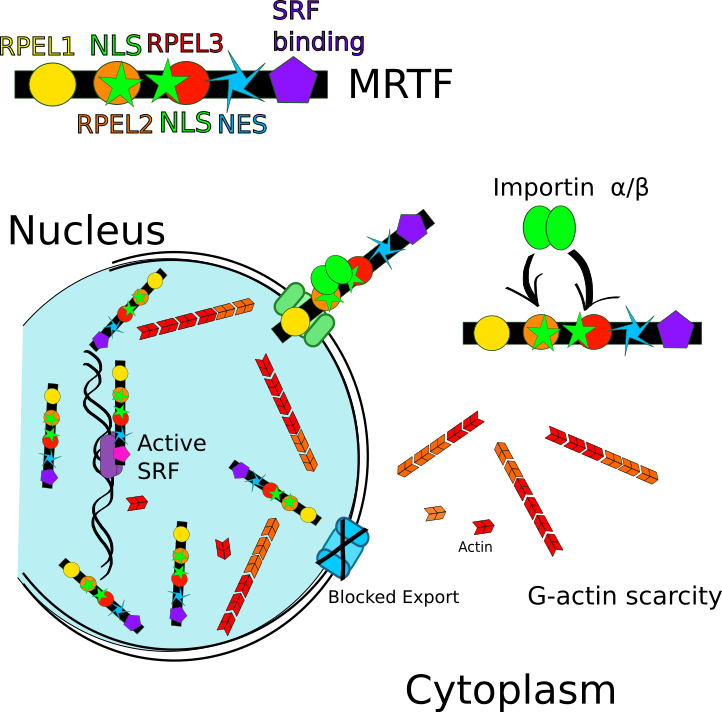
\includegraphics[scale=0.45]{Figures/Nuclear.png} 
\hline
\vspace{0.2cm}
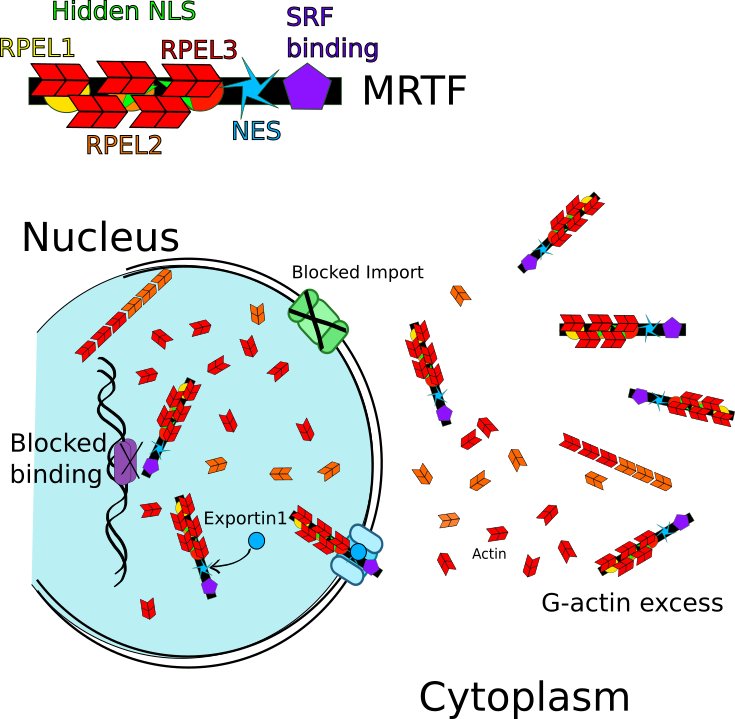
\includegraphics[scale=0.45]{Figures/Cyto.png} 
\caption{Résumé de la localisation de MRTF-A en fonction de la quantité de monomères d'actine disponible}
\end{figure}

\chapter{Rhéologie locale d'une cellule unique}
\begin{figure}[p]
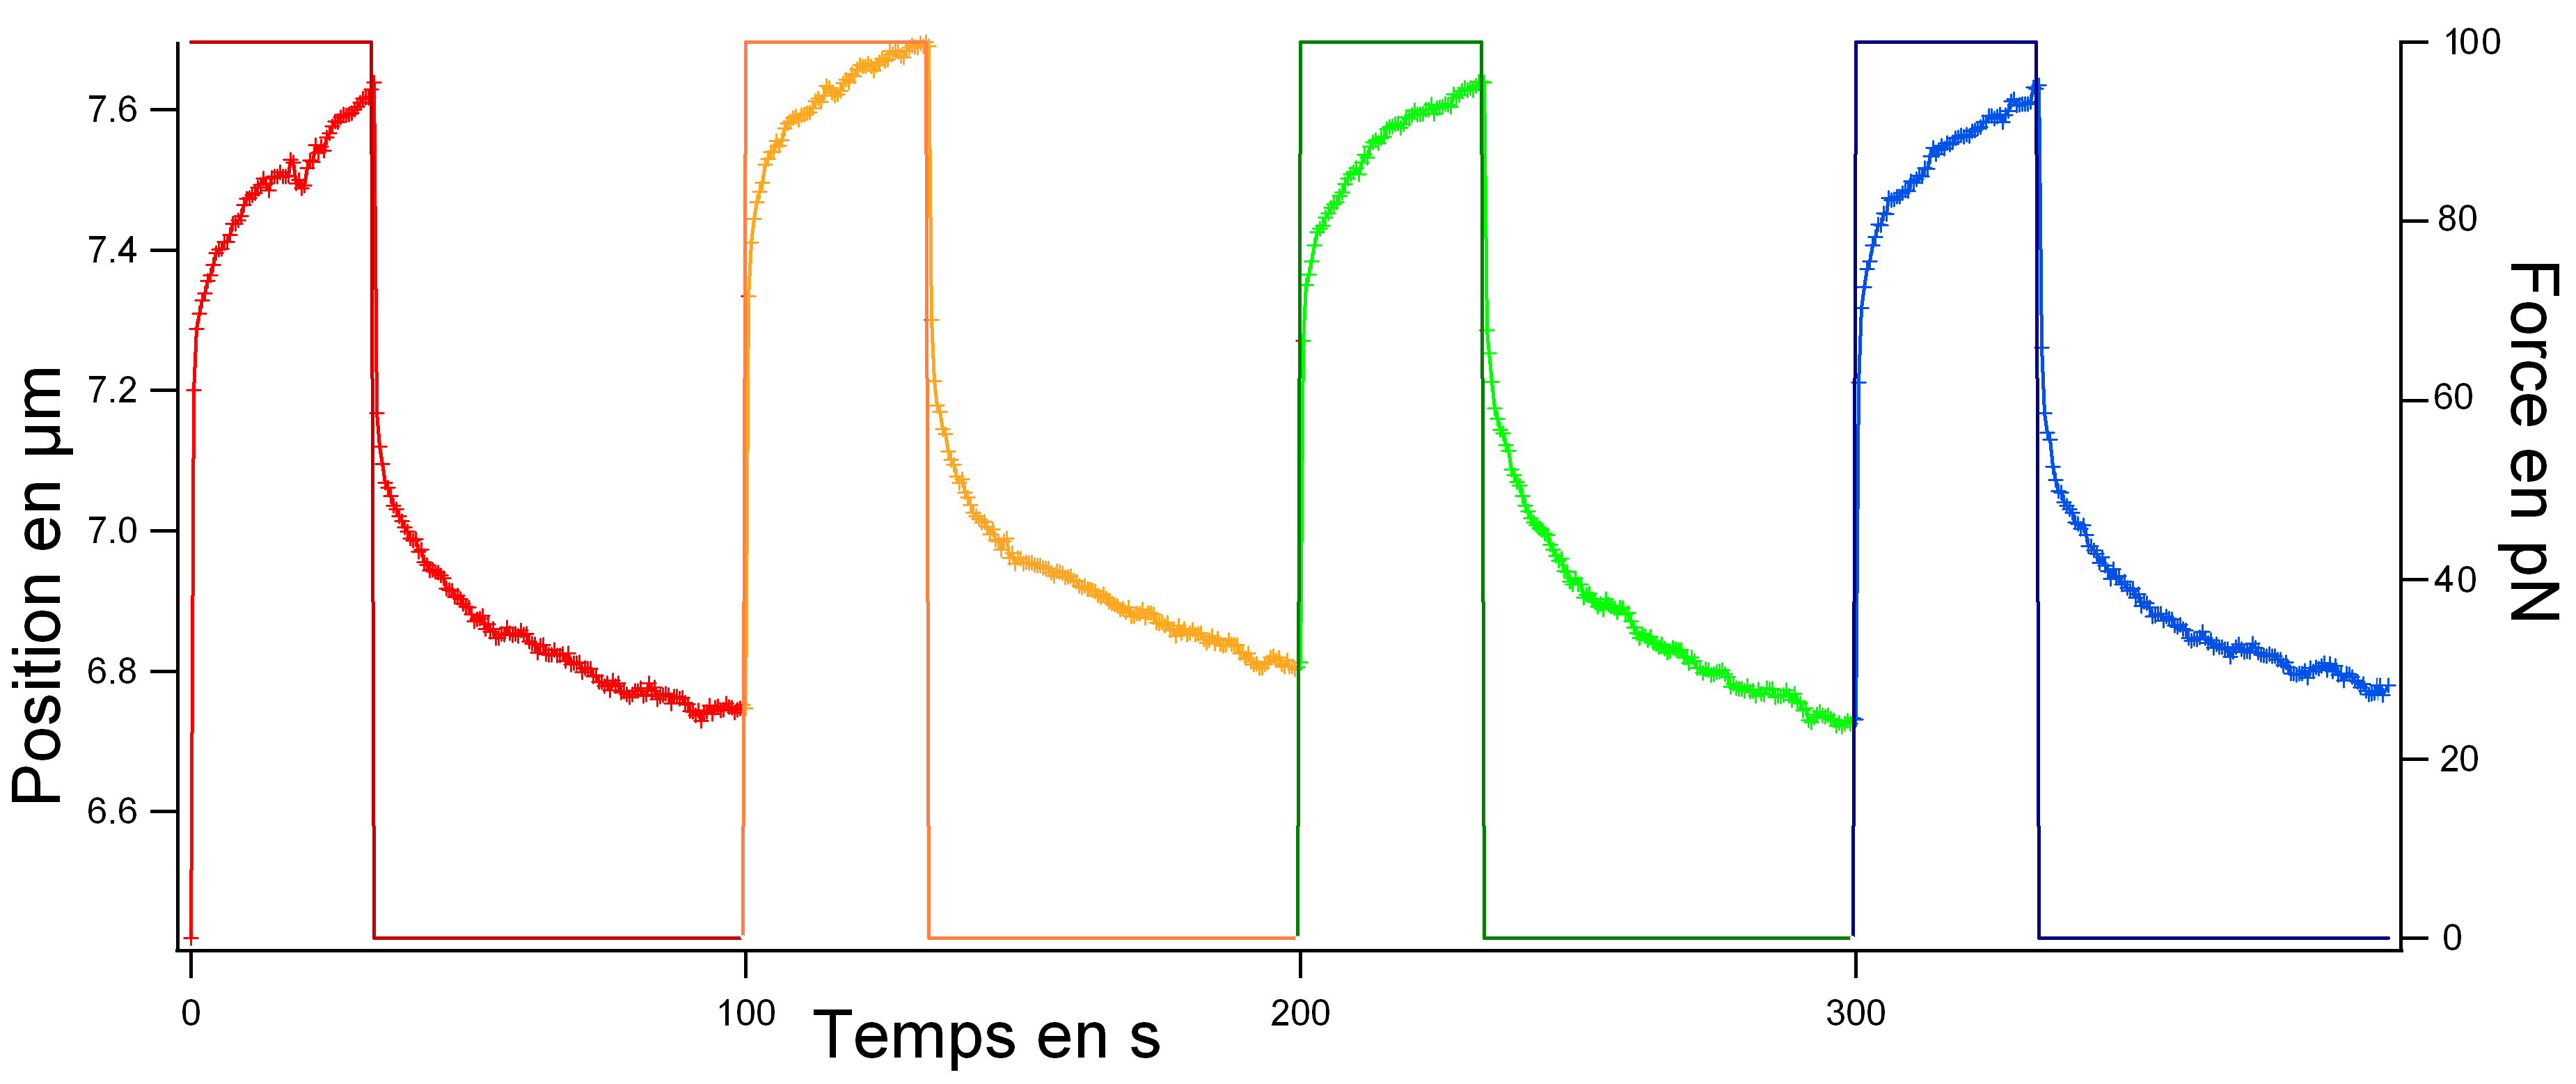
\includegraphics[scale=0.09]{c9-rigidification-couleurs.png}

\caption{Exemple de tracé de la position selon $x$ d'une bille au cours du temps lorsqu'elle est soumise à 4 créneaux de force successifs. $\delta R(t)$ =$\delta x(t)$ lorsque le déplacement ne se fait que selon l'axe $X$.\label{Exemple}} 
	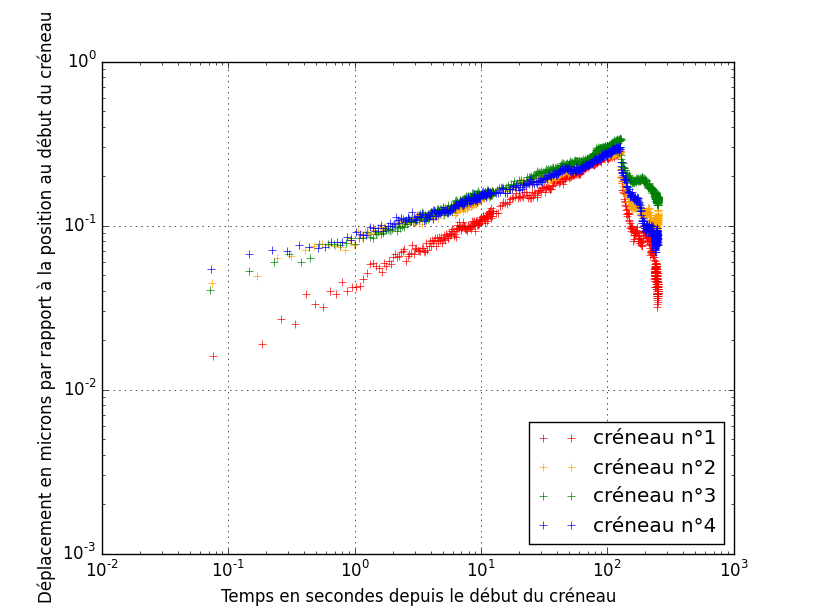
\includegraphics[scale=0.5]{Figures/Exemple_C162_loglog.png}
	\caption{Déplacement de la bille en fonction du temps écoulé depuis le début du créneau, pour les 4 créneaux successifs. On peut remarquer l'allure caractéristique en loi de puissance. On peut également voir qu'ici qu'après le premier créneau le déplacement est plus grand en réponse à la même force : la cellule s'est \og ramollie \fg. }
\end{figure}

\begin{figure}[p]
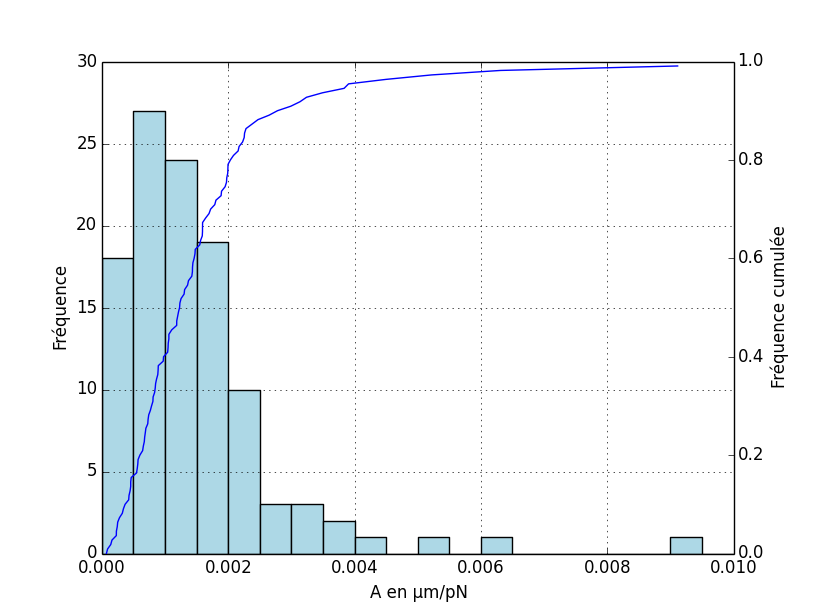
\includegraphics[scale=0.5]{Figures/A0_Toutes.png} 
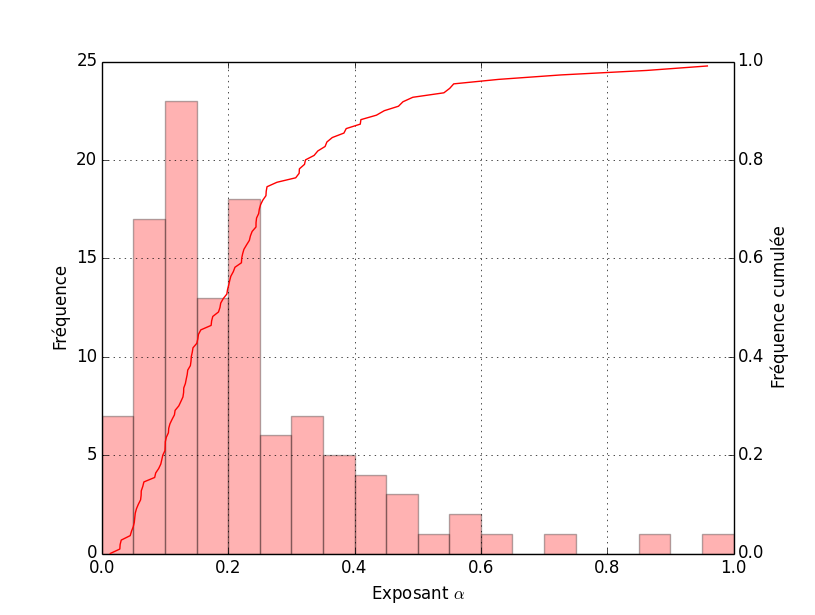
\includegraphics[scale=0.5]{Figures/E0_Toutes.png} 
\caption{Caractéristiques mécaniques des C2C12 sondées par des billes fonctionnalisées avec 4 \micro g de fibronectine.}
\end{figure}

\begin{figure}[p]
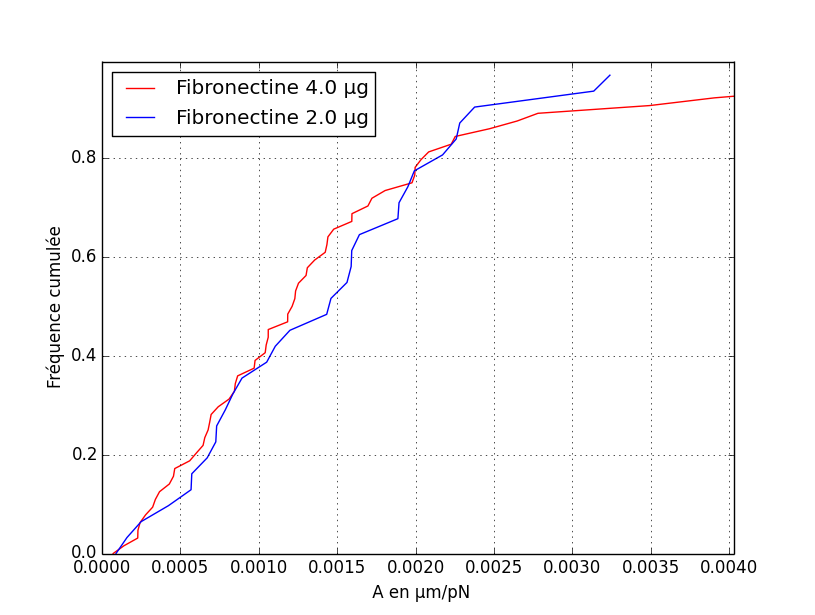
\includegraphics[scale=0.5]{Figures/A_coating_seul.png} 
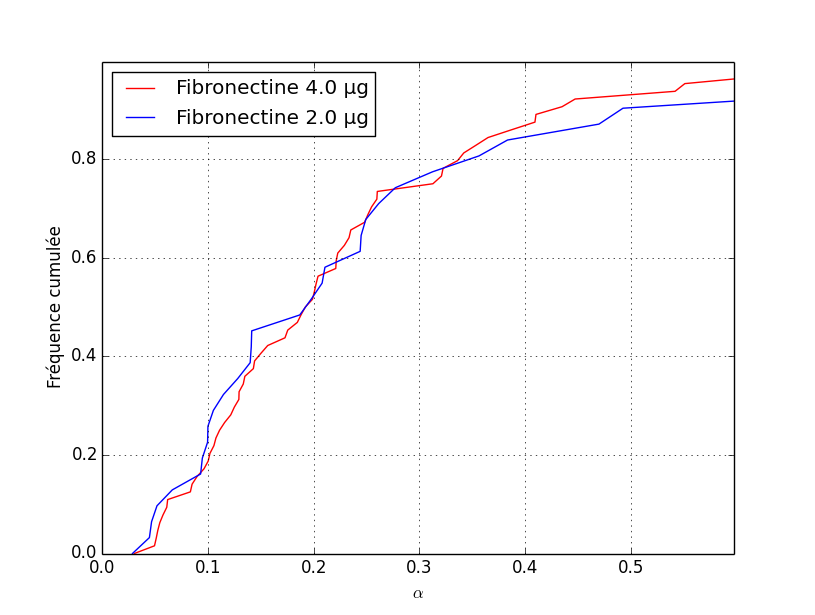
\includegraphics[scale=0.5]{Figures/E_coating_seul.png} 
\caption{Caractéristiques des C2C12 sondées par des billes ayant différentes densités de fibronectine à leur surface. (p=0.13 avec un test de Student comparant les deux distributions). }
\end{figure}

\begin{center}
\begin{figure}[p]
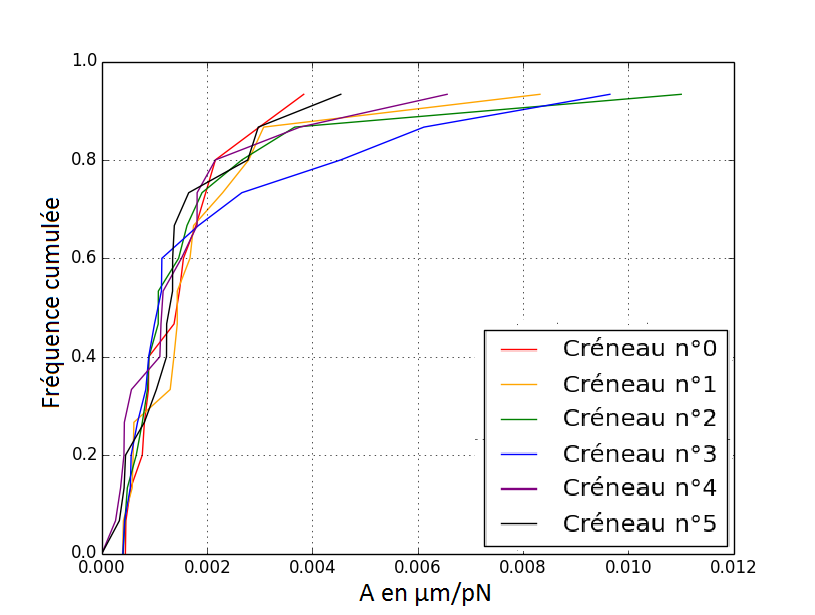
\includegraphics[width=6.5cm]{Figures/A_creneaux_temoin.png}
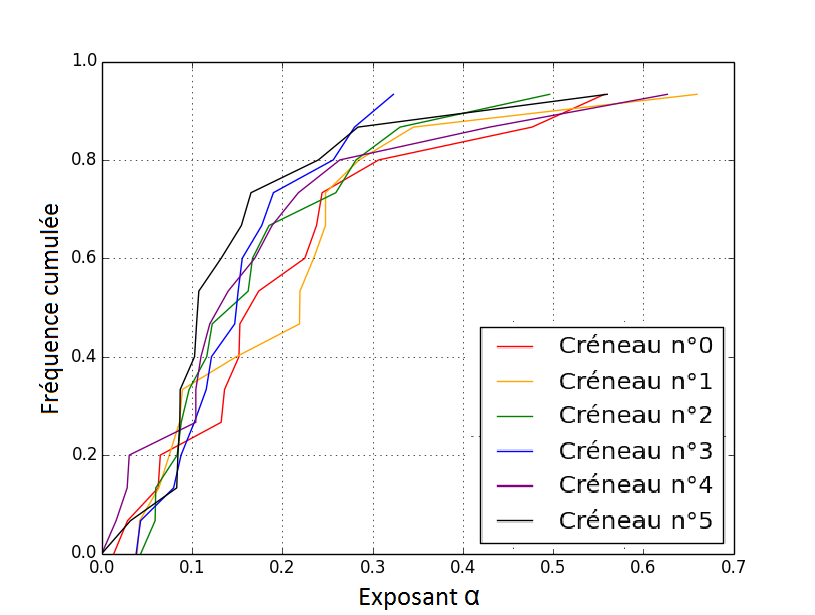
\includegraphics[width=6.5cm]{Figures/E_creneaux_temoin.png} 

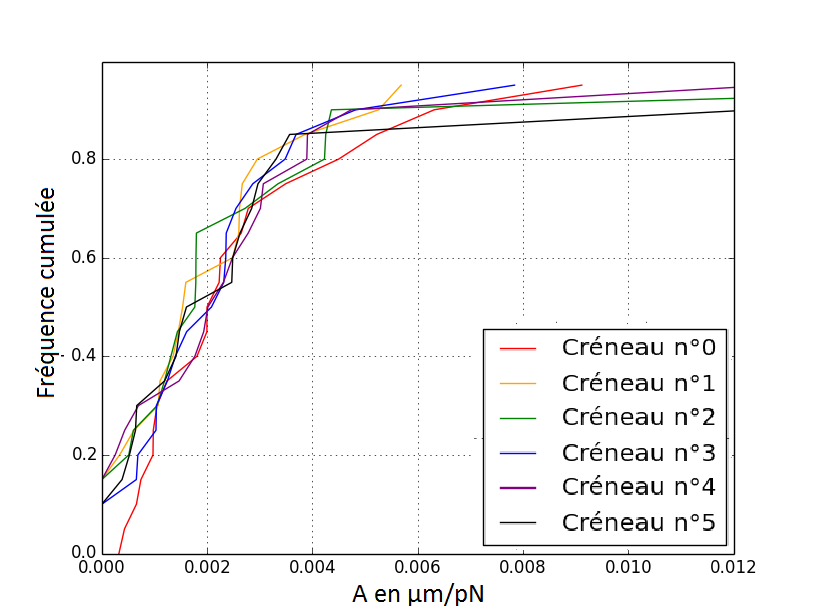
\includegraphics[width=6.5cm]{Figures/A_creneaux_S2.png} 
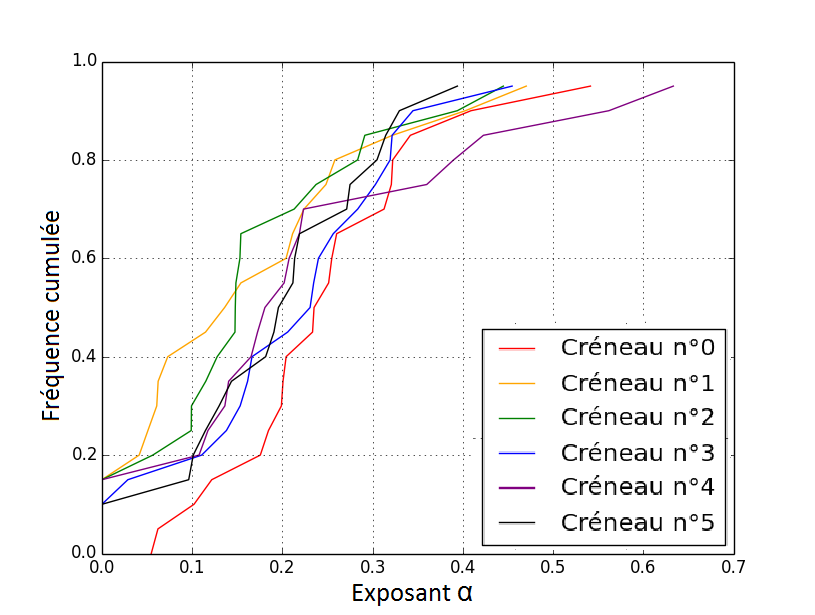
\includegraphics[width=6.5cm]{Figures/E_creneaux_S2.png} 
\caption{\label{Evolution_6c} Histogramme des paramètres $A$ et $\alpha$ pour six applications de force successives, pour le témoin avec 10s d’application de force, en haut, et pour 125s d’application de force, en bas.}
\end{figure}
\end{center}
\begin{figure}[p]
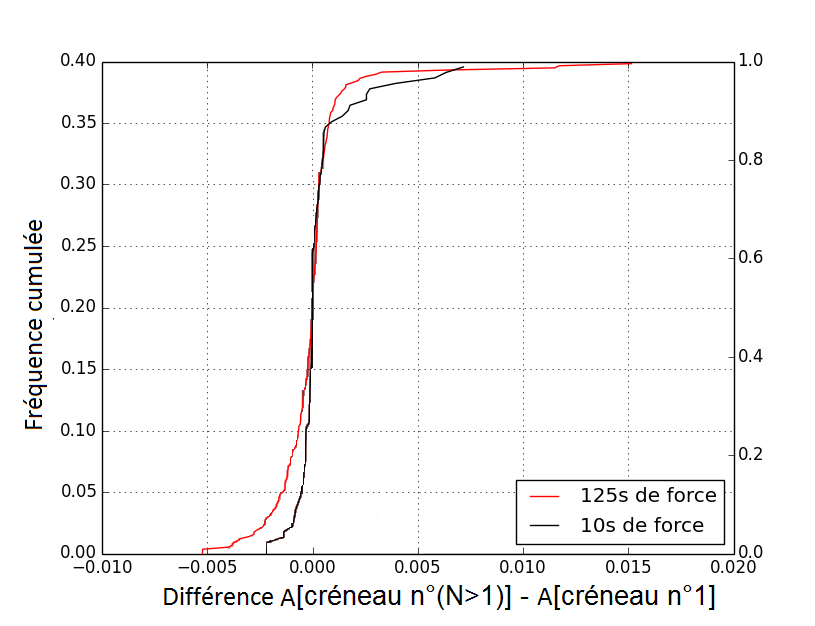
\includegraphics[height=5cm]{Figures/A_diff_seul.png} 
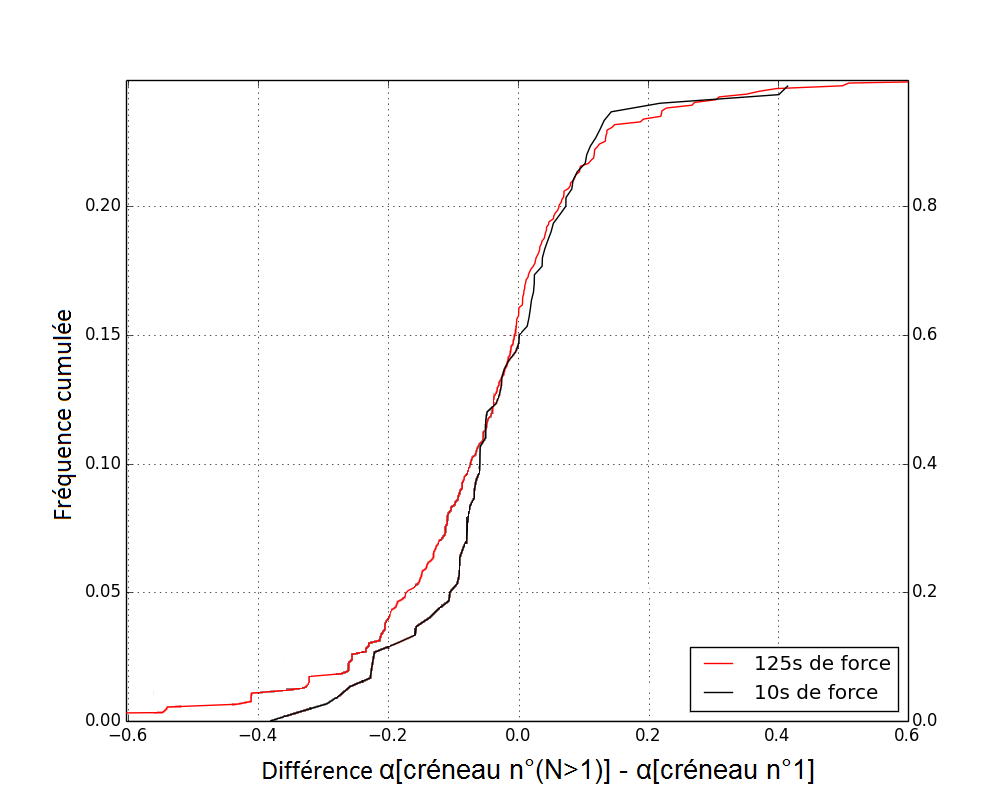
\includegraphics[height=5cm]{Figures/E_diff_seul.png}
\caption{Amplitude des évolutions de A entre la première mesure et les 6 suivantes, pour la série témoin (10s de force, en noir) et pour la même concentration de fibronectine et 125s de force (en rouge).}
\label{Diff}
\end{figure}

\begin{figure}[p]
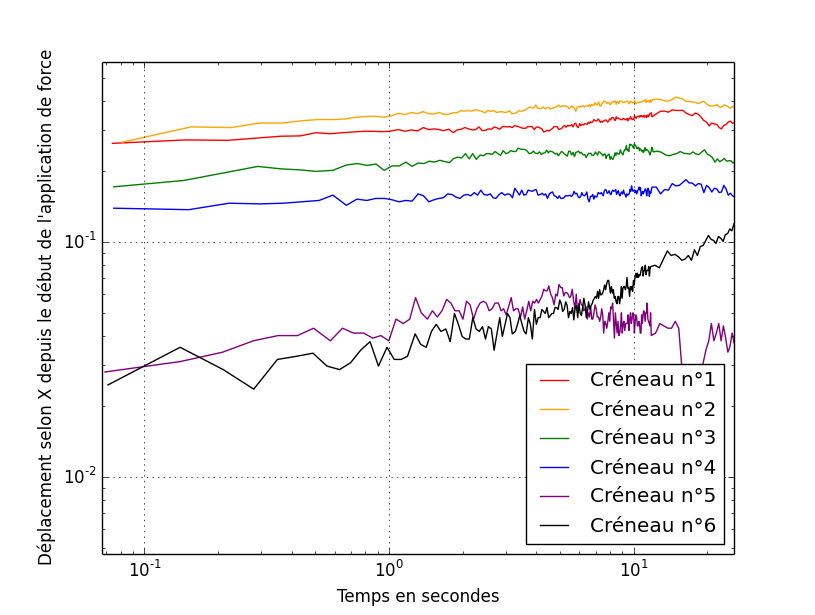
\includegraphics[scale=0.33]{Figures/Rigidification_exemple_s2c2.png} 
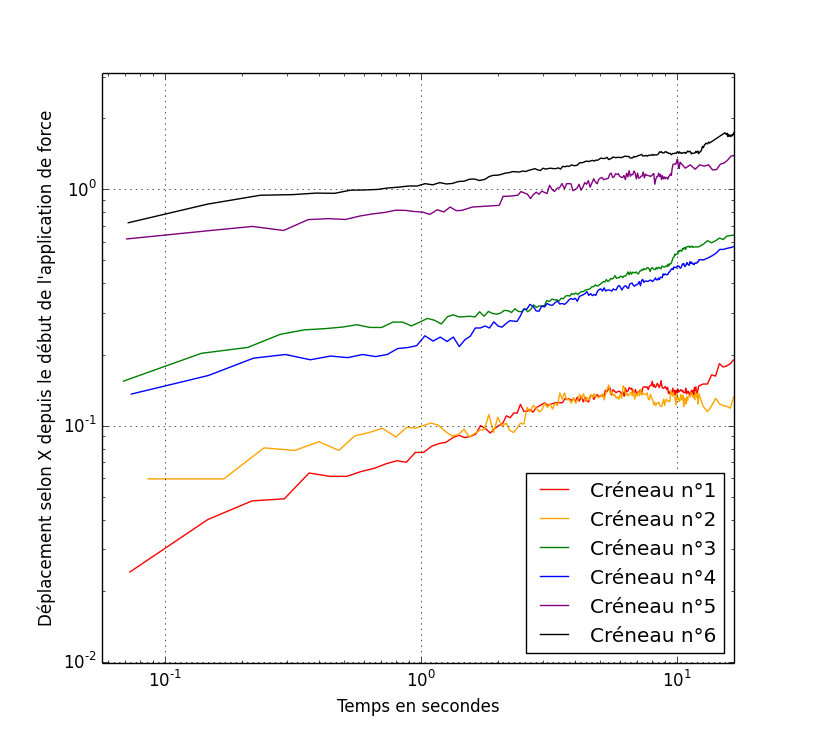
\includegraphics[scale=0.3]{Figures/Ramollissement_exemple_s2c19.png} 
\caption{Exemples de déplacements au cours du temps et au cours des applications de forces d'une cellule considérée comme en rigification (à gauche) et d'une cellule en ramollissement (à droite)}
\end{figure}

\begin{figure}[p]
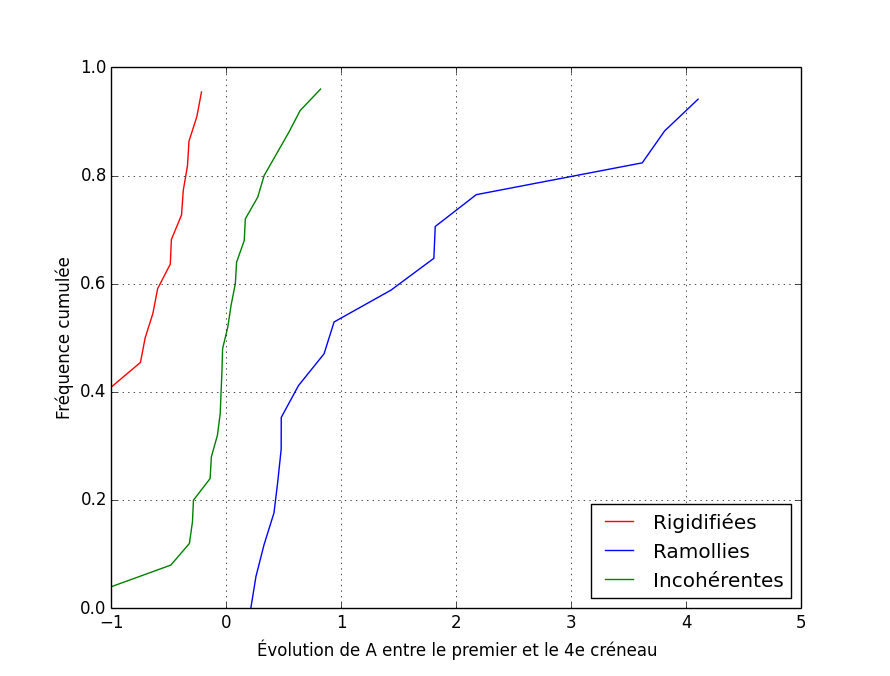
\includegraphics[width=10cm]{Figures/Evolution_J4-J0_sur_J0.png} 
%AXE DES x A REMPLACER PAR : EVOLUTIONS RELATIVES DE A ENTRE ….
\caption{Histogrammes cumulés de $\frac{A_4-A_1}{A_1}$ pour les trois groupes de cellules classées. On voit que près de la moitié des cellules se rigidifiant sont passées sous le seuil de détection de la pince, tandis que les ramollissements sont souvent supérieurs à 100\%.  }
\end{figure}

\begin{figure}[p]
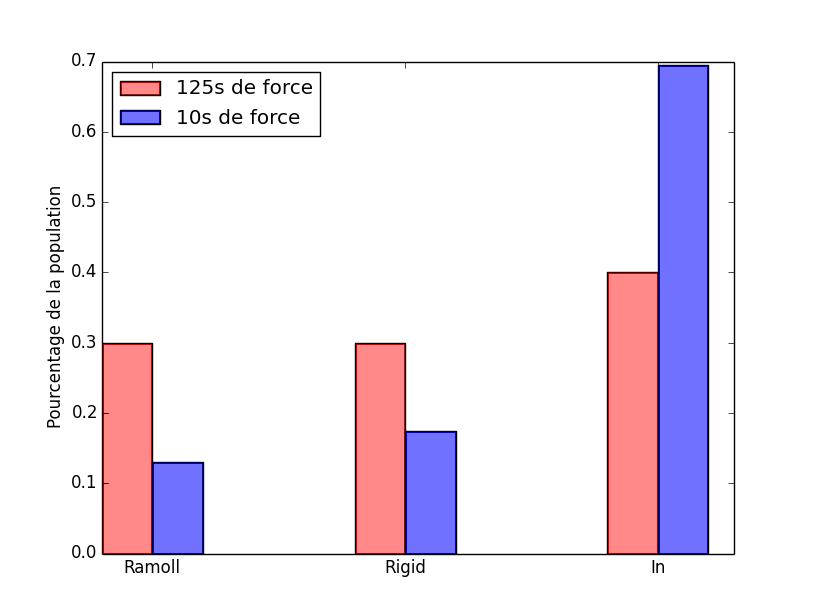
\includegraphics[width=10cm]{Figures/FRI_temoin_vs_C4.png} 
\caption{Répartition des cellules dans les trois catégories d'évolution de $A$ au cours des applications de force \label{FRI_temoin}}
\end{figure}

\begin{figure}[p]
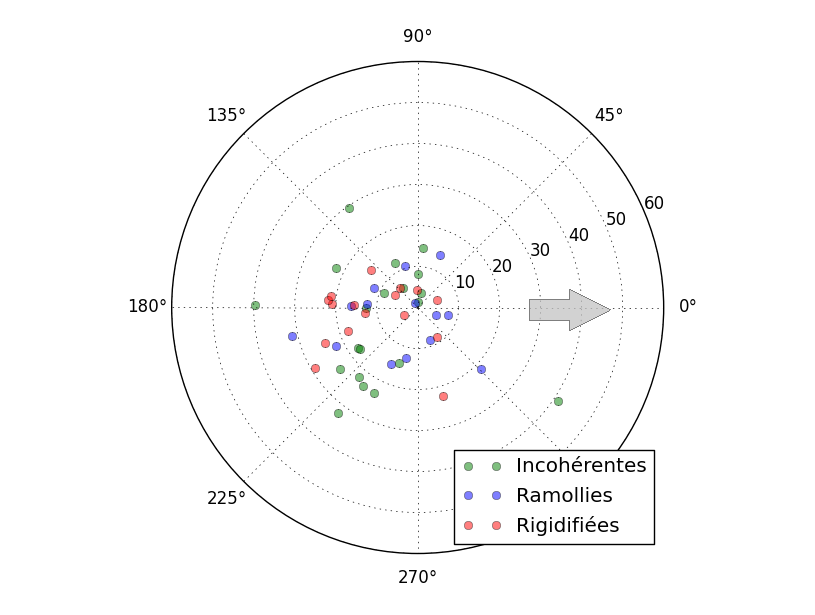
\includegraphics[scale=0.45]{Figures/Positions_FRI.png} 
\caption{Longueur et orientation du vecteur entre le bord du noyau et la bille. La flèche représente la direction de la force exercée sur les billes.\label{polar}}
\end{figure}
\begin{figure}[p]
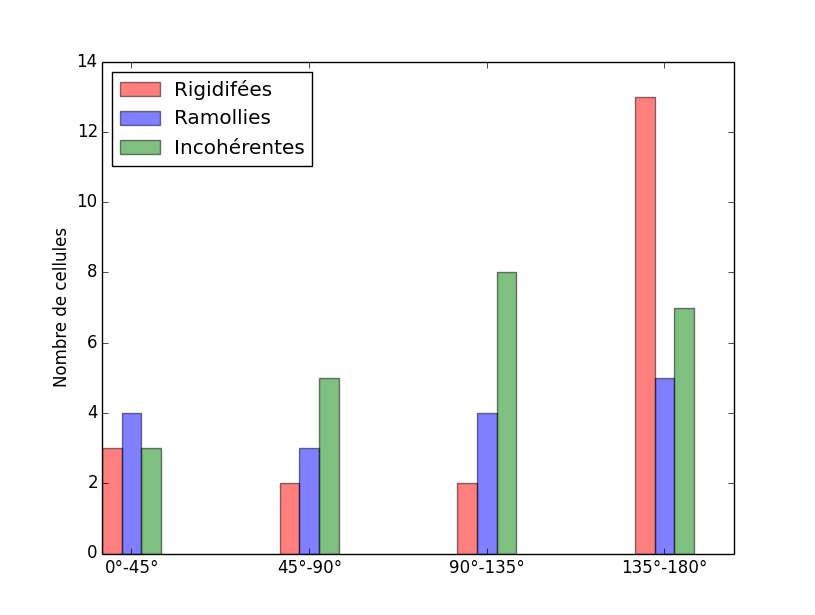
\includegraphics[scale=0.45]{Figures/Hist_Angles.png} 
\caption{Répartition des comportements cellulaires en fonction de l'angle formé entre l'axe bille-noyau et la direction de la force appliquée, pour 125 secondes de force et 4 \micro g de fibronectine. (Le test de Fisher donne p=0.044 pour que cette distribution soit due au hasard.) \label{Angle_C4}}
\end{figure}
\begin{figure}[p]
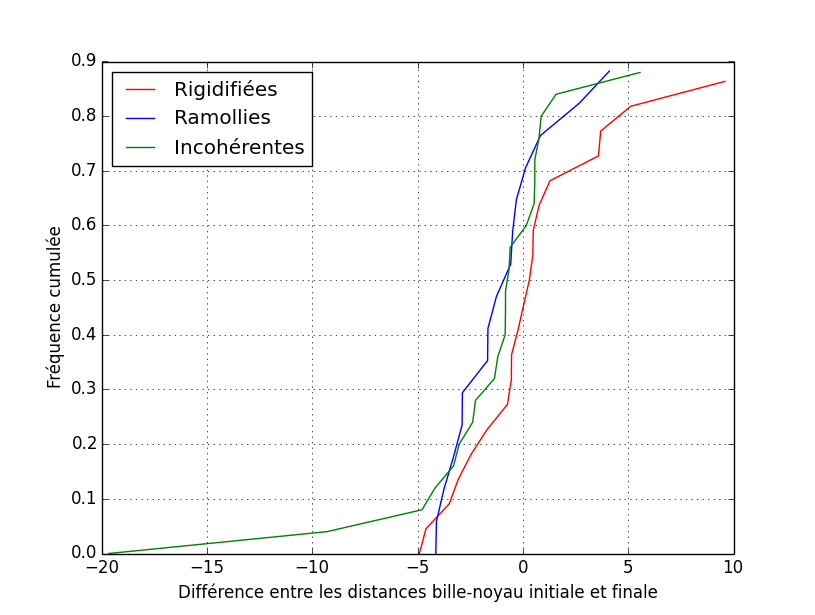
\includegraphics[scale=0.45]{Figures/Evolution_DBN.png}
\caption{Différence entre la distance bille-noyau finale et la distance bille-noyau initiale, pour les cellules classées précédemment. \label{DBN}}
\end{figure}

 \begin{figure}[p]
\caption{\small Résultats des expériences sur les E-cadhérines mutantes incapables d'interactions \textit{cis}, d'après \cite{Strale}. A : Montage expérimental, B : Proportion des billes immobiles, mobiles ou arrachées sous force pour des cellules exprimant la cadhérine mutante (cis Ecad, 54 cellules) ou sauvage (wt Ecad, 39 cellules). C : Déplacements des billes sous force en fonction du temps. D : Moyennes des déplacements pour toutes les applications de force, pour 12 billes dans chaque condition. E : Trajectoires (en \micro m) d'une bille pendant les six périodes de relaxation dans les deux conditions. F : Déplacement quadratique moyen pendant la relaxation pour 12 billes et 6 créneaux dans chaque condition}
\end{figure} 
     
 \begin{figure}[p]
 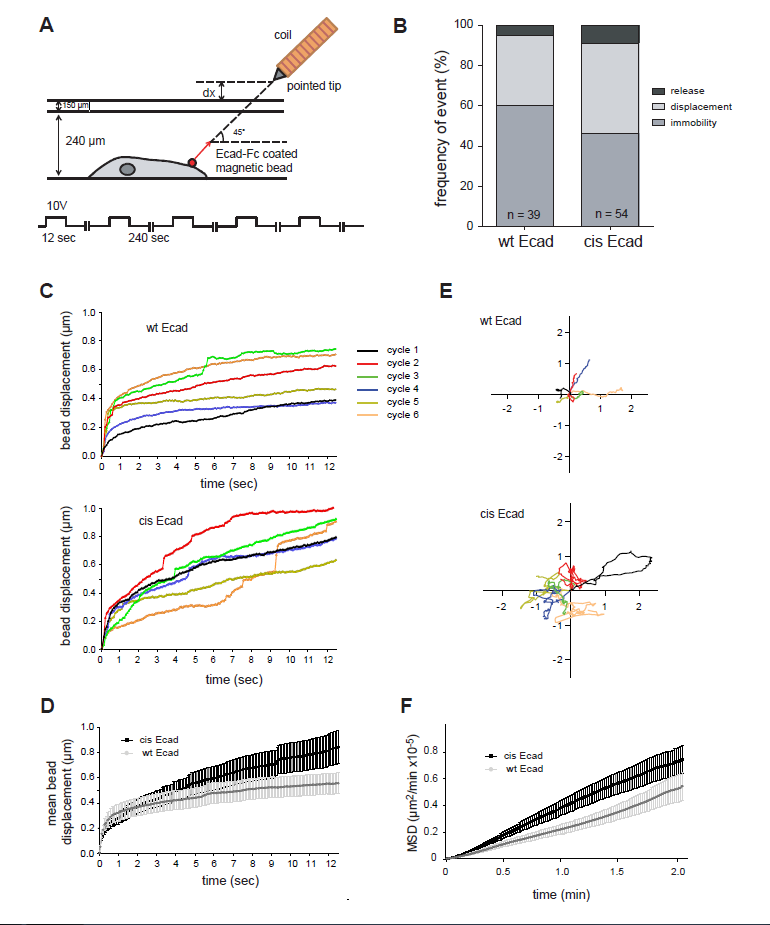
\includegraphics[scale=0.7]{Figures/Strale.png} 

 \end{figure}
 
 \chapter{Changement de localisation de MRTF-A dans les cellules musculaires en réponse à une stimulation mécanique}
 
  \begin{figure}[p]
  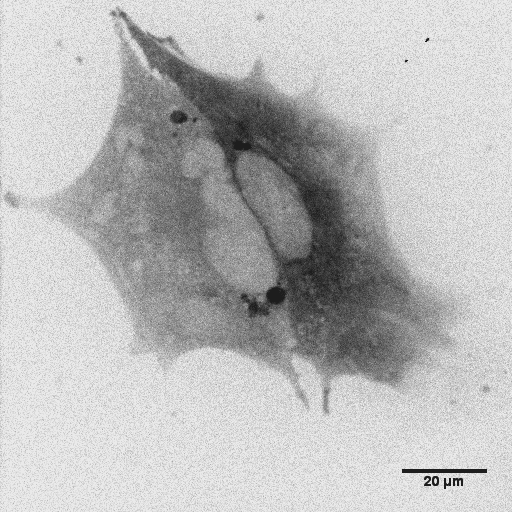
\includegraphics[width=3.5cm]{Figures/Exemple_C_GFP_impress.png} 
 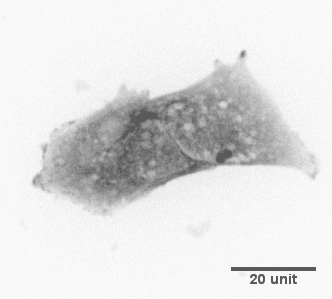
\includegraphics[width=3.5cm]{Figures/Exemple_H_GFP_impress.png} 
 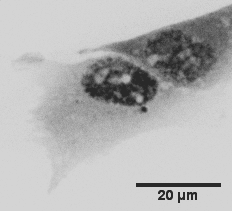
\includegraphics[width=3.5cm]{Figures/Exemple_N_2_GFP_impress.png} 
 \caption{Exemples de cellules classées comme MRTF-A Cytoplasmique, Homogène et Nucléaire, de gauche à droite respectivement. En bleu, la phalloïdine marquant les filaments d'actine, en jaune la MRTF-A GFP.\label{Exemples_CHN}}

 \end{figure}
 
 \begin{figure}[p]
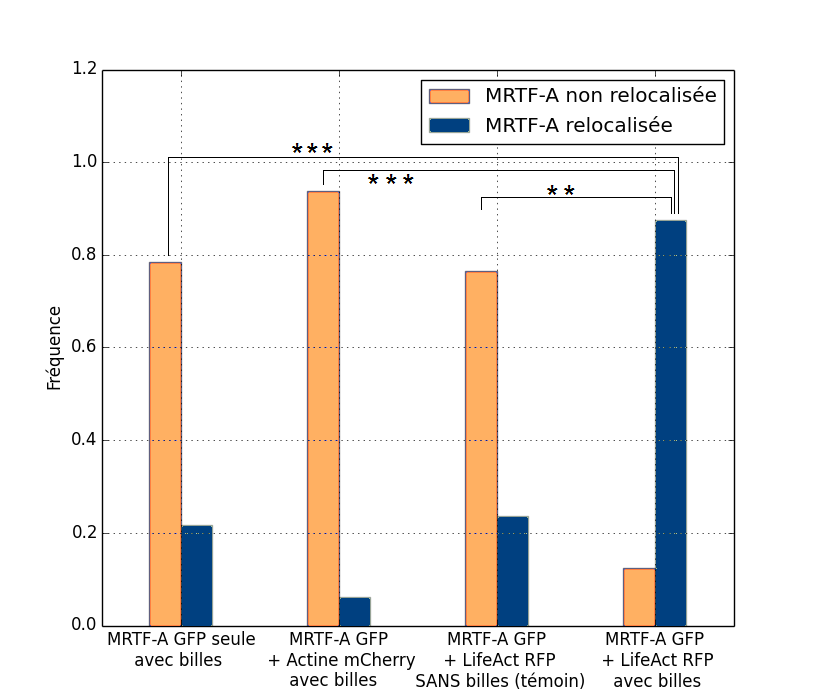
\includegraphics[scale=0.4]{Figures/Pinces_MRTFA_stars_colors.png} 
\caption{Proportion des cellules observées pour lesquelles MRTF-A GFP change de localisation dans la cellule au cours de l'expérience. * : $p<\frac{0.05}{4}$ , ** $p<\frac{0.01}{4}$, *** $p<\frac{0.001}{4}$ (réalisés avec un test de Fisher et une correction pour les comparaisons multiples)\label{MRTF-A Pinces}}
\end{figure}

\begin{figure}[p]
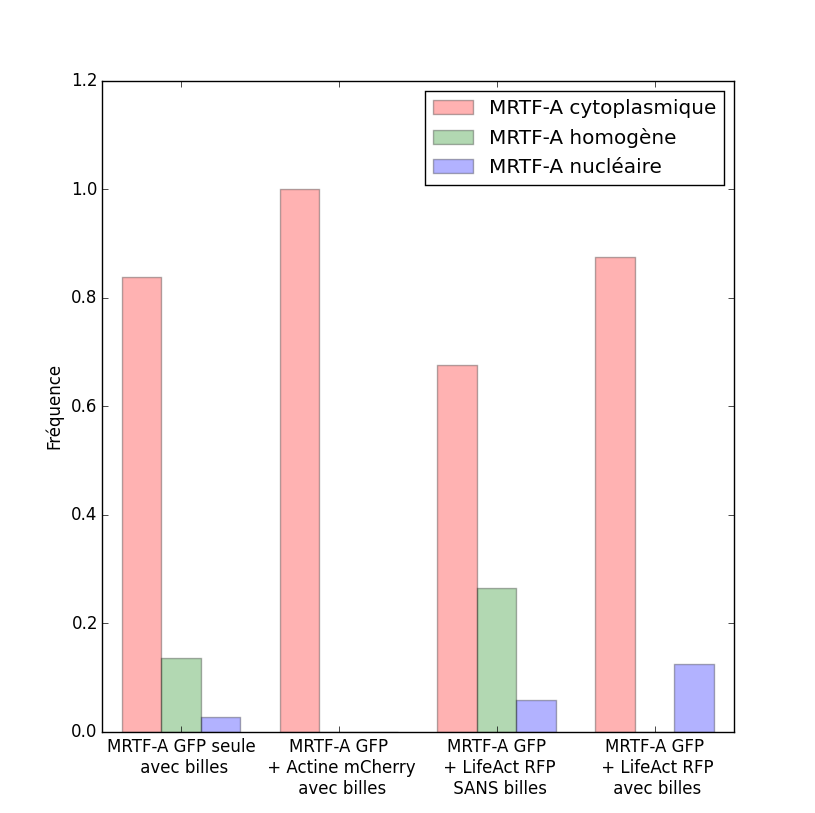
\includegraphics[scale=0.4]{Figures/CHN_pinces.png} 
\caption{Répartition de MRTF-A dans les cellules avant application de la force. \label{CHN_pinces}}
\end{figure}

\begin{figure}[p]
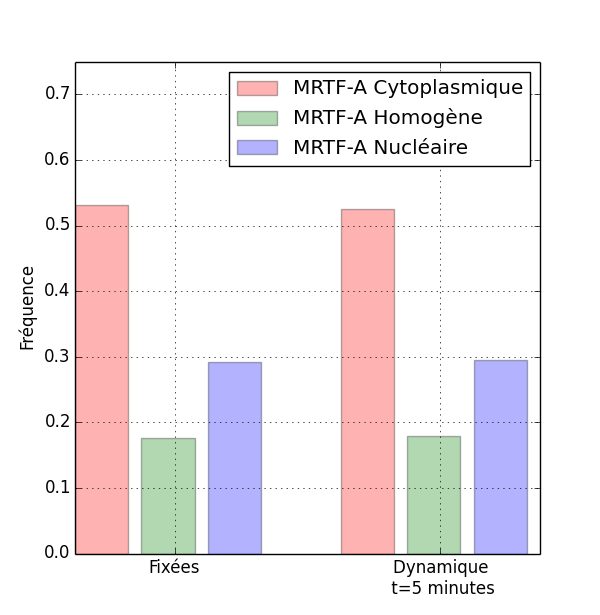
\includegraphics[scale=0.5]{Figures/Reference.png} 
\caption{Répartition entre les trois états pour des cellules fixées immédiatement après un montage sans rinçage et sans étirement (n=7, 963 cellules) et lors de l'observation en direct après 5 minutes d'observation sans étirement (n=5, 41 cellules). La différence n'est pas significative (p=0.995, G-test).
\label{Référence}}
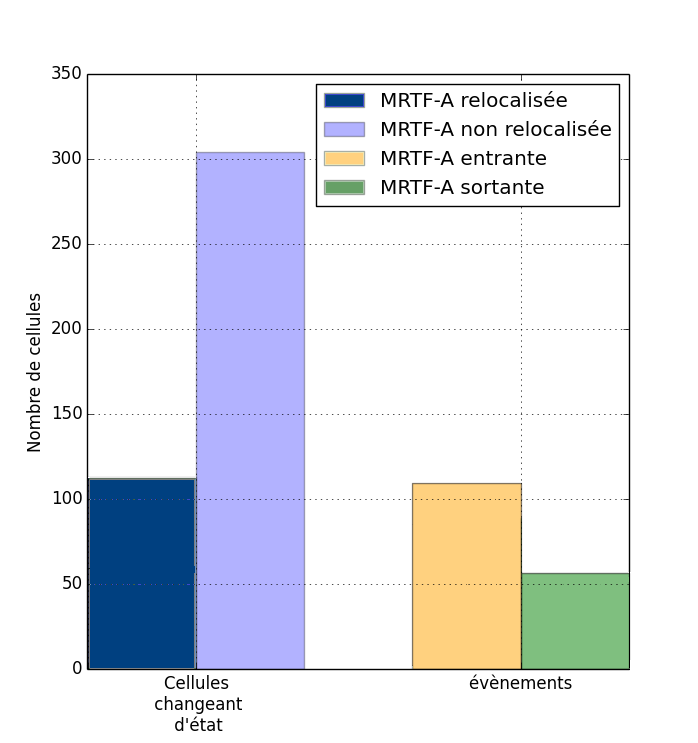
\includegraphics[scale=0.4]{Figures/Reference_transloc.png} 
\caption{Quantité de cellules changeant au moins une fois d'état pendant 2 heures d'observation et direction de ces changements \label{Ref_transloc}}
\end{figure}

\begin{figure}[p]
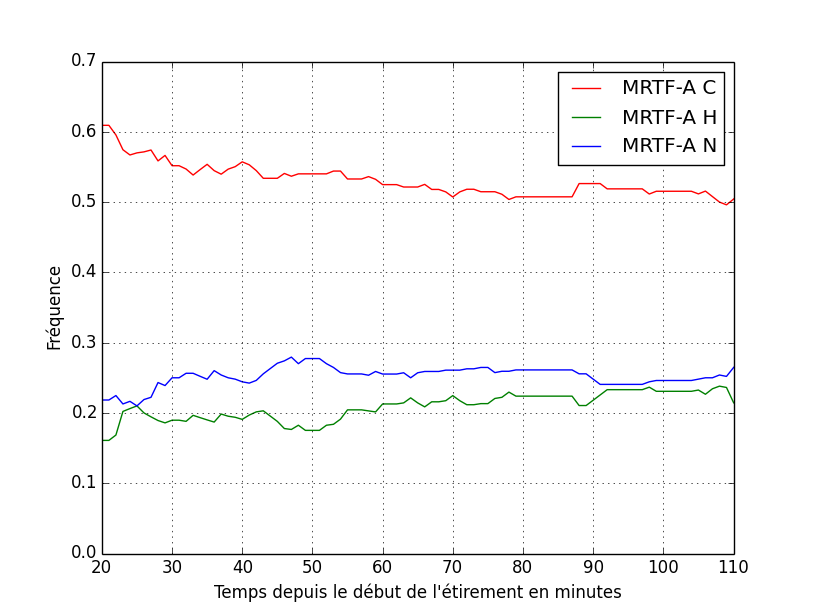
\includegraphics[scale=0.4]{Figures/CHN_vs_Temps_reference.png} 
\caption{\label{Reference_dynamique} \'E{}volution de la proportion de cellules ayant MRTF-A dans chacune des trois localisations au cours du temps lors d'une expérience témoin où l'on a monté à l'avance la lamelle dans l'étireur et où l'on n'applique aucune contrainte.}
\end{figure}


\begin{figure}[p]
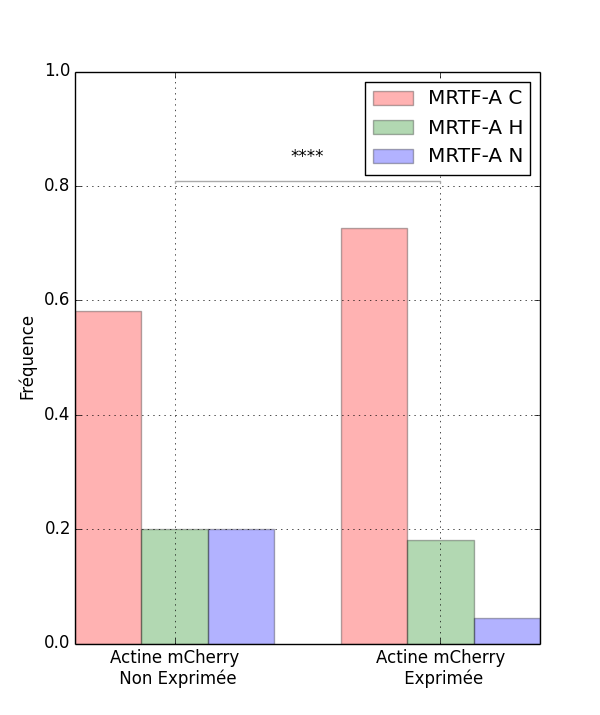
\includegraphics[scale=0.4]{Figures/AMC.png}
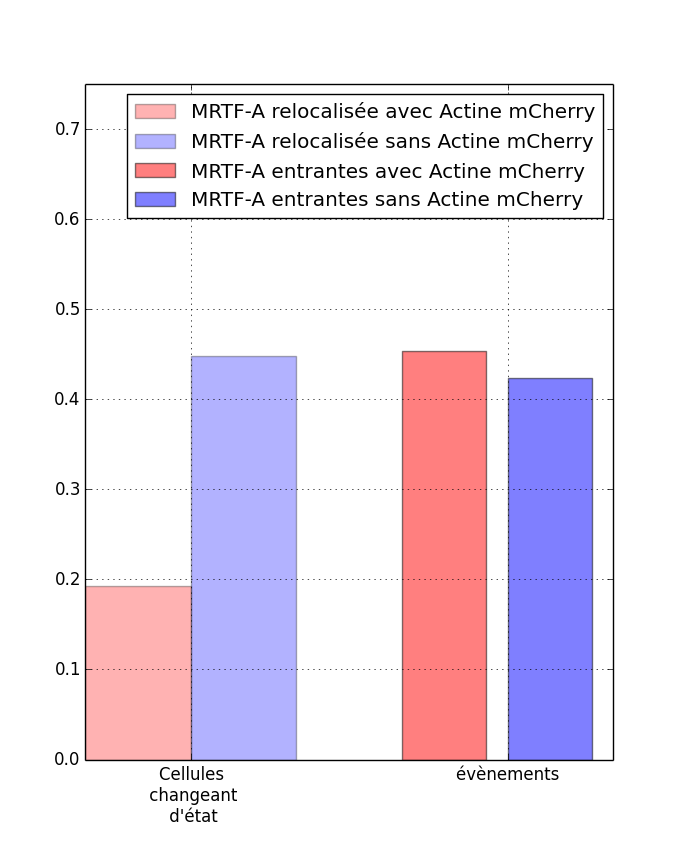
\includegraphics[scale=0.3]{Figures/AMC_translob.png}
\caption{\label{AMC}Répartition initiale pour des cellules issues des mêmes expériences exprimant ou non le plasmide Actine mCherry (683 cellules témoin et 538 cellules expriment l'Actine mCherry). **** : $p<10^{-4}$}\caption{\label{AMC_transloc}Proportion de cellules changeant au moins une fois d'état et proportion d'entrantes et de sortantes, pour les même expériences, selon que l'Actine mCherrry est exprimée ou non.}
\end{figure}

\begin{figure}[p]
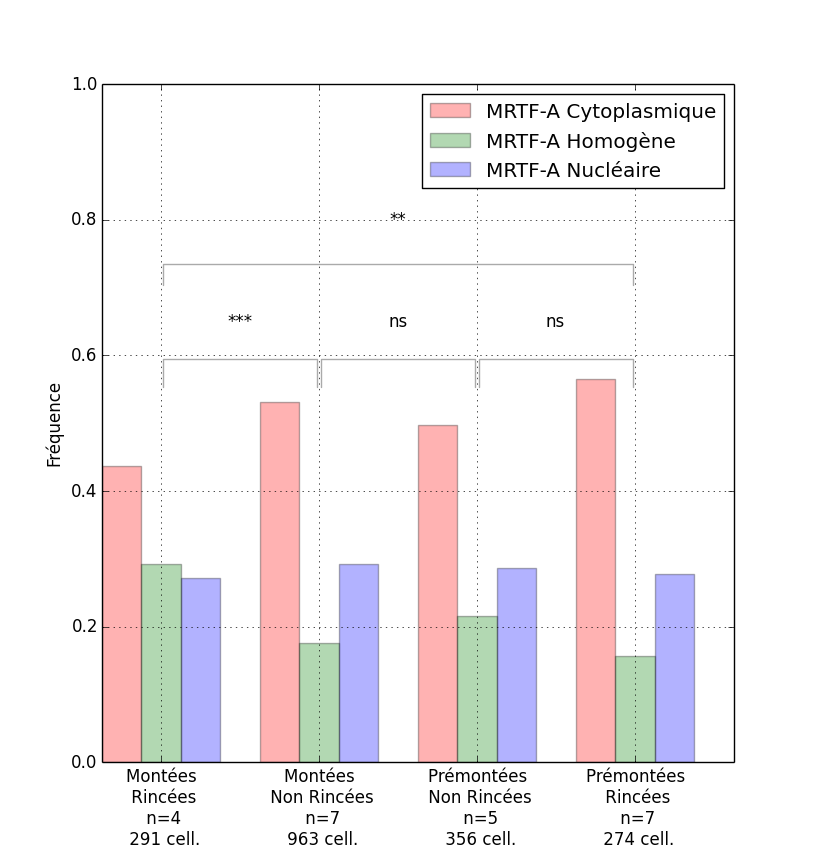
\includegraphics[scale=0.5]{Figures/CHN_montage_rincage.png} 
\caption{\label{CHN_montage} Influence sur la localisation de MRTF-A des contraintes mécaniques dues au montage de la lamelle dans l'étireur (Montage) et de la variation de concentration en sérum due au remplacement du milieu de culture par du milieu neuf au moment du montage (Rinçage). Montées : montage à $t-5$ minutes, Prémontées : montage à $t-18$ heures, rinçage au même moment.
Tous les tests on été réalisés avec un G-test d'indépendance t et une correction de Bonferroni pour les comparaisons multiples. ** : $p<\frac{0.01}{4}$ et *** : $p<\frac{0.001}{4}$}
\end{figure}

\begin{figure}[p]
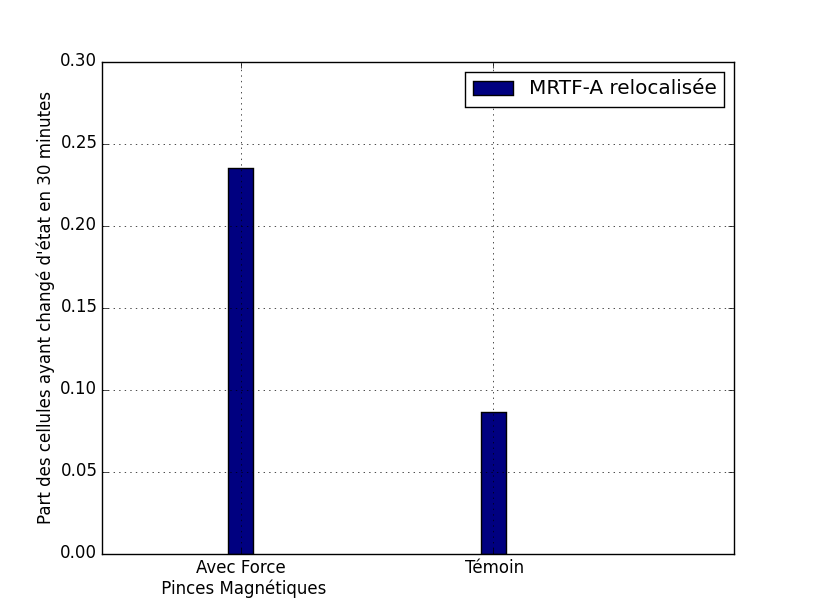
\includegraphics[scale=0.4]{Figures/Pinces_vs_temoin.png} 
\caption{\label{pinces_vs_temoin} Proportion des cellules observées pour lesquelles MRTF-A GFP change de localisation dans la cellule au cours de l'expérience. p=0.012 (G-test d'indépendance)}
\end{figure}

\begin{figure}[p]
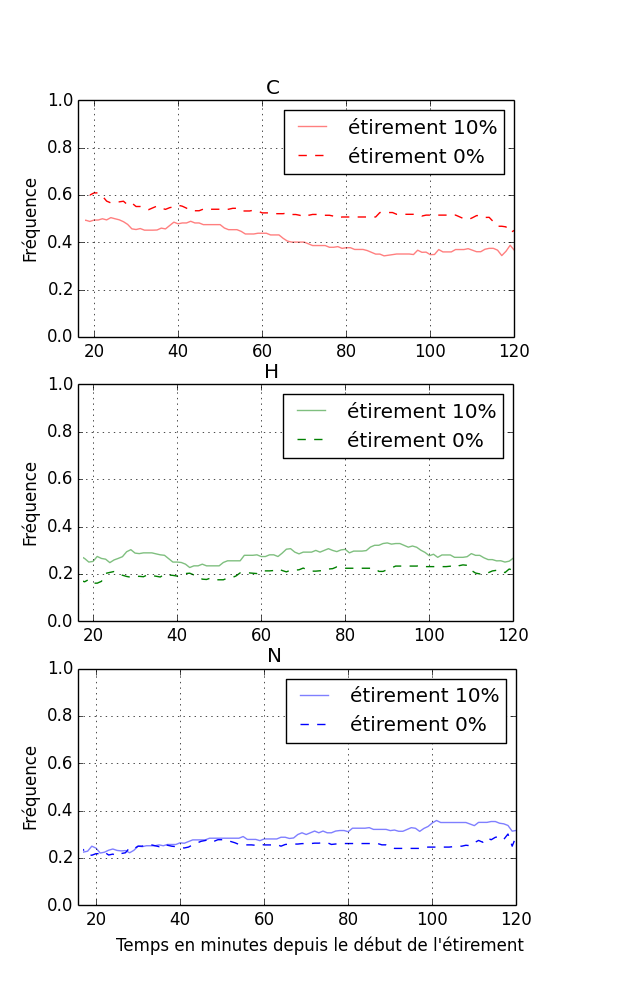
\includegraphics[scale=0.4]{Figures/Etirement10_vs_0_dynamique.png} 
\caption{\label{CHN_dyn_Et10} Comparaison de l'évolution de la fréquence de chaque localisation de MRTF-A au cours du temps après 10\% d'étirement et dans les expériences témoin (n=5 et 141 cellules dans les deux cas)}
\end{figure}

\begin{figure}[p]
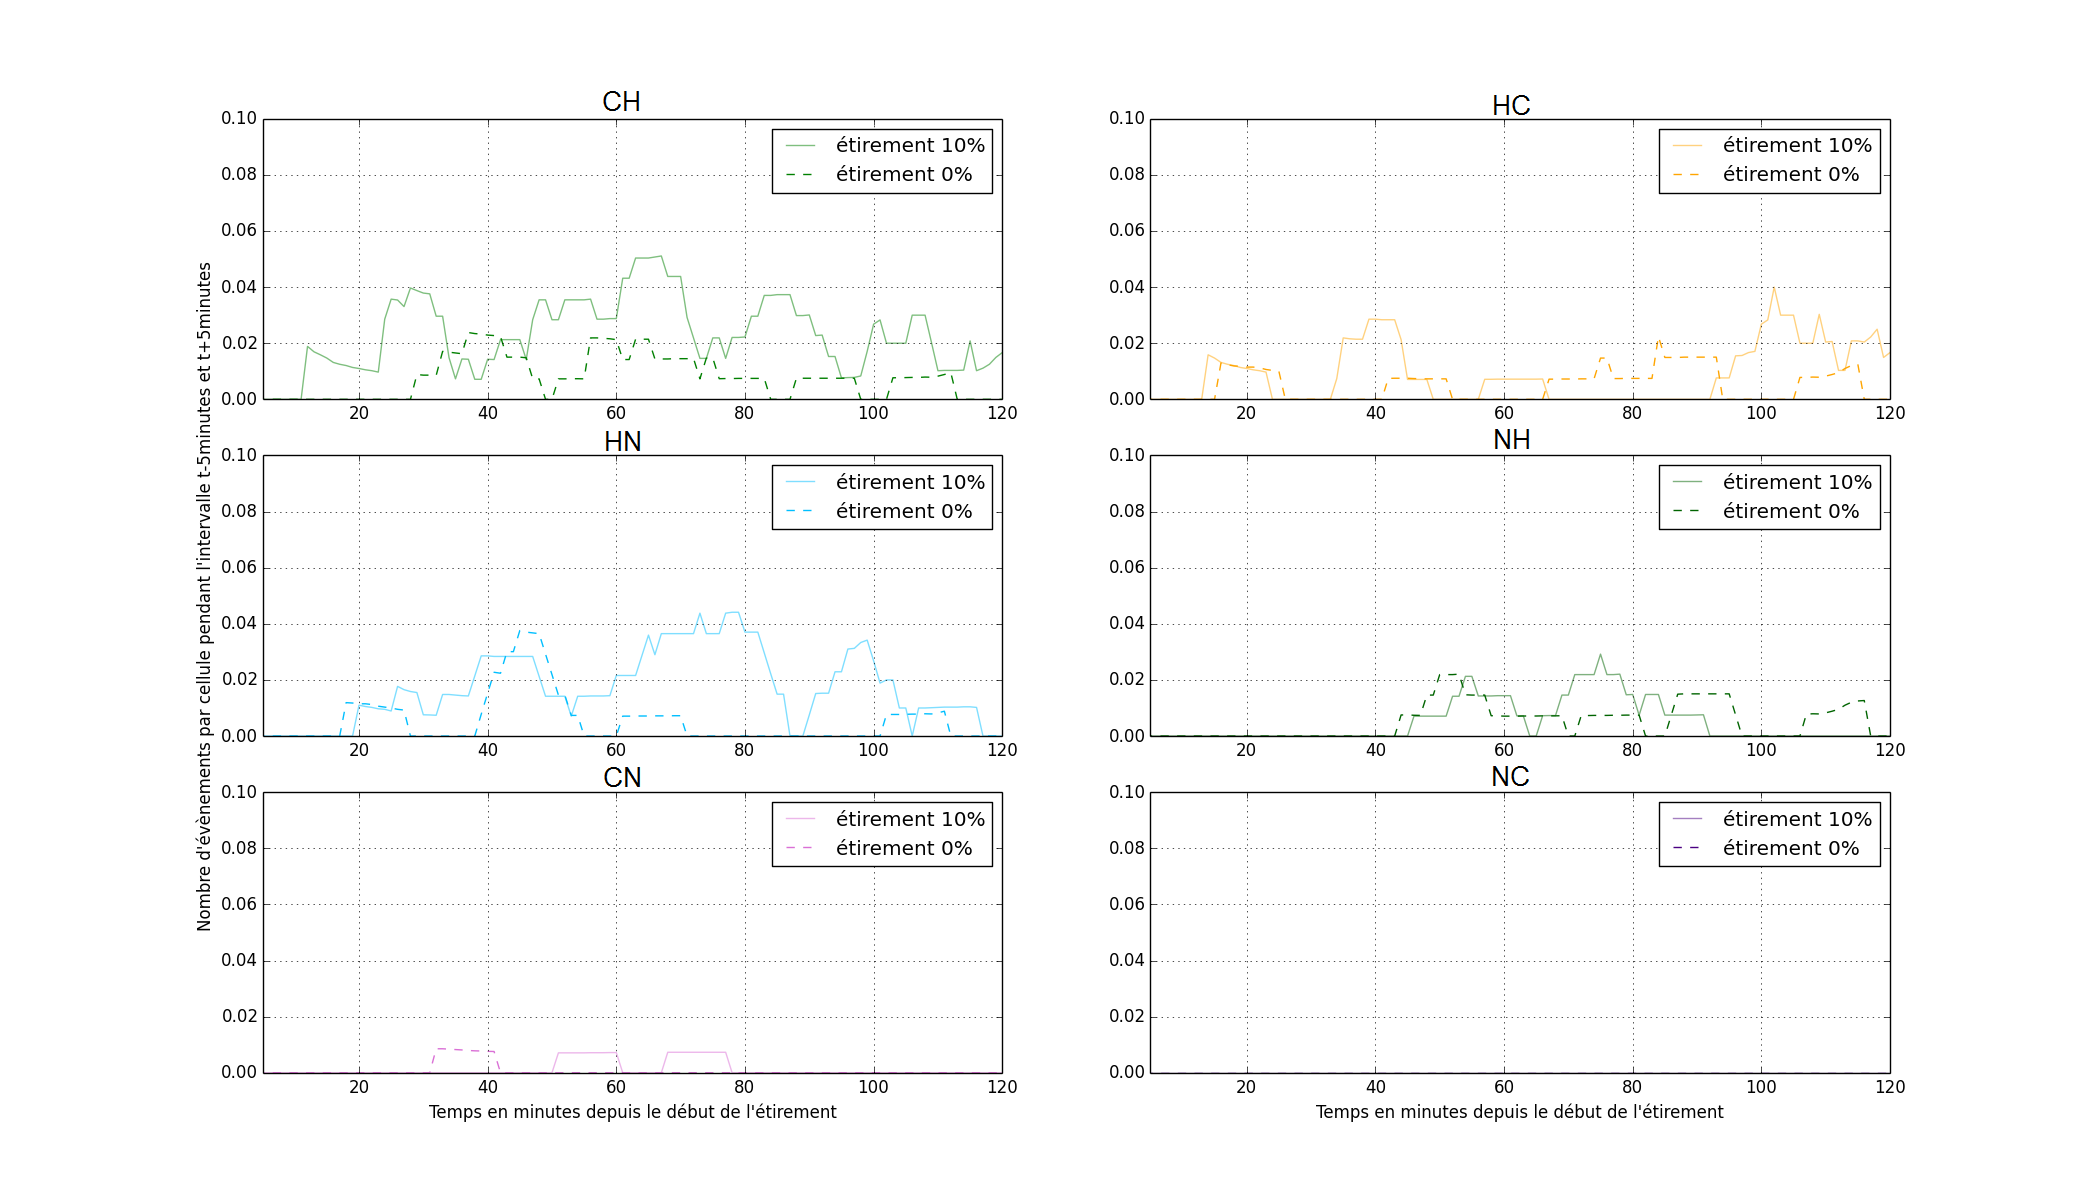
\includegraphics[scale=0.33]{Figures/Etirement10_vs_0_translocations.png} 
\caption{\label{transloc_dyn_Et10} Nombre d'évènements ayant eu lieu pendant la fenêtre [t-5min,t+5min] pour chaque type de transition possible divisé par le nombre de cellules observées. La première lettre du titre de chaque graphe représente l'état initial de la localisation de MRTF-A dans la cellule, la seconde lettre l'état final. Par exemple le premier graphe "CH" représente le nombre de cellules dans lesquelles MRTF-A est passée d'une localisation cytoplasmique à homogène dans l'intervalle [t-5min;t+5min] divisé par le nombre total de cellules.}
\end{figure}

\begin{figure}[p]
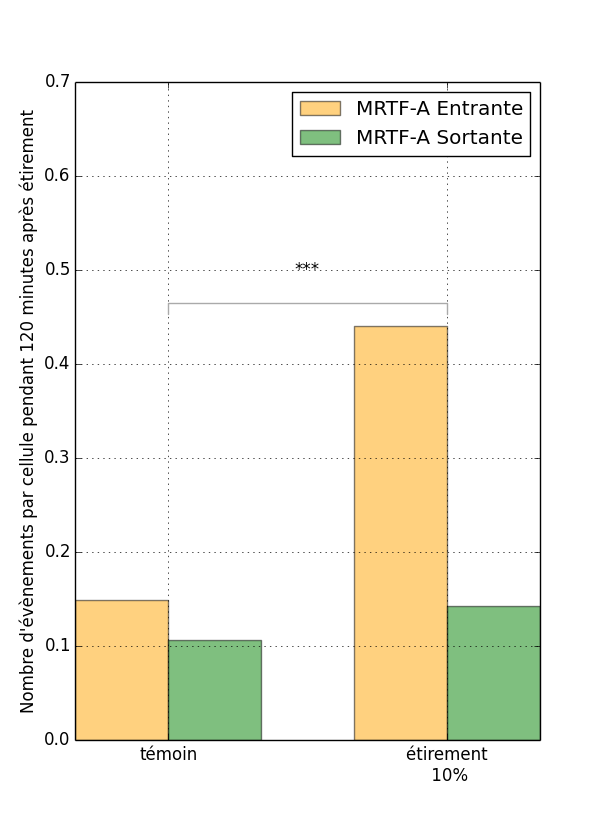
\includegraphics[scale=0.4]{Figures/Etirement10_vs_temoin_activite.png} 
\caption{\label{activite_Et10} Nombre d'évènements entrants ou sortants par cellule observée pendant 120 minutes, pour l'étirement 10\% et pour le témoin. p=0.0003 }
\end{figure}

\begin{figure}[p]
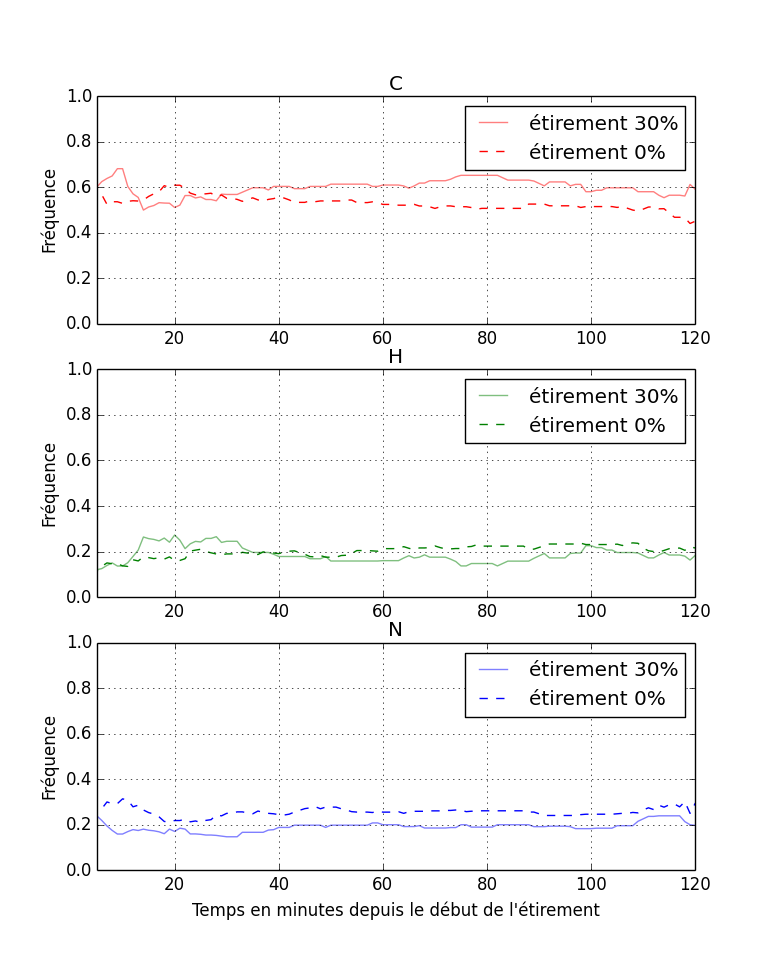
\includegraphics[scale=0.5]{Figures/Etirement30_vs_0_dynamique.png} 
\caption{\label{Et30_CHN} Comparaison de l'évolution de la fréquence de chaque localisation de MRTF-A au cours du temps après 30\% d'étirement ou dans les expériences témoin (n=5 et 141 cellules pour le témoin, n=3 et 102 cellules pour l'étirement 30\%)}
\end{figure}

 
\begin{figure}[p]
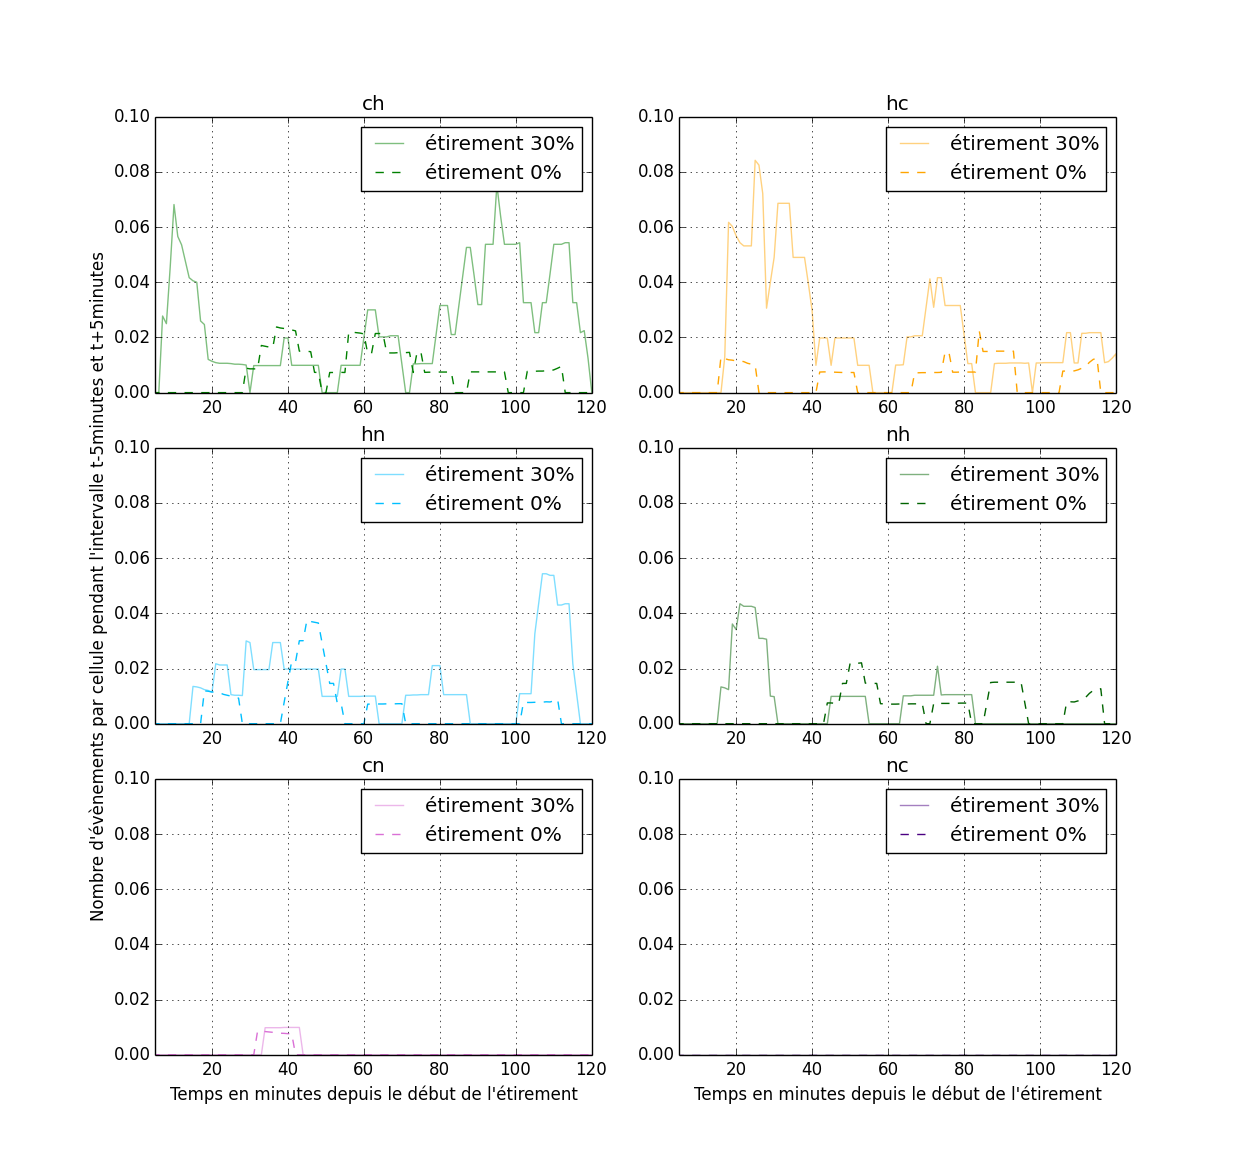
\includegraphics[scale=0.5]{Figures/Etirement30_vs_0_translocations.png}
\caption{\label{Et30_transloc} Nombre d'évènements ayant eu lieu pendant la fenêtre [t-5min,t+5min] pour chaque type de transition possible divisé par le nombre de cellules observées. La première lettre du titre de chaque graphe représente l'état initial de la localisation de MRTF-A dans la cellule, la seconde lettre l'état final. Par exemple le premier graphe "CH" représente le nombre de cellules dans lesquelles MRTF-A est passée d'une localisation cytoplasmique à homogène dans l'intervalle [t-5min;t+5min] divisé par le nombre total de cellules. }
\end{figure}

\begin{figure}[p]
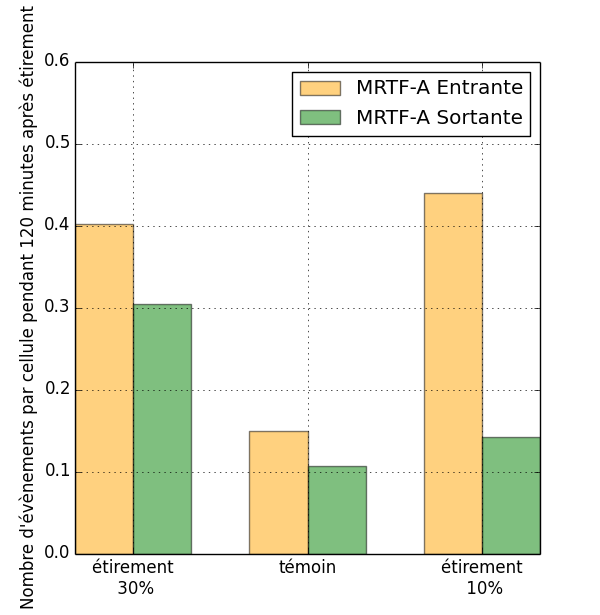
\includegraphics[scale=0.5]{Figures/Etirement30_vs_temoin_activite.png}
\caption{\label{Et30_activite} Quantité de changements d'état par cellule pour les trois conditions différentes (p=$10^{-4}$, G-test d'indépendance).}
\end{figure}

\begin{figure}[p]
 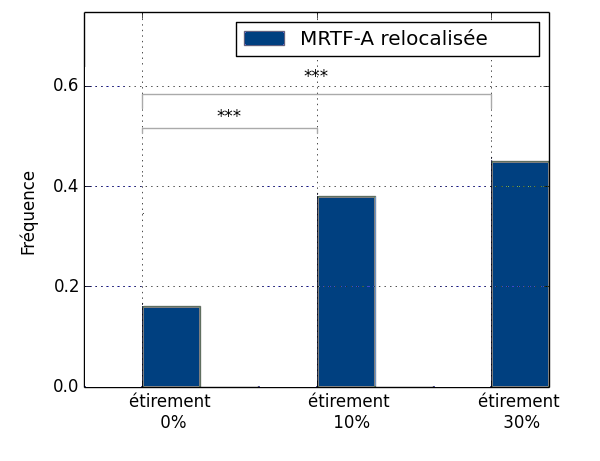
\includegraphics[scale=0.5]{Figures/Activite.png} 
 \caption{\label{Et30_ES} Comparaison pour les deux étirements et le témoin de la proportion de cellules qui changent d'état au moins une fois}
 \end{figure}
 
 \begin{figure}[p]
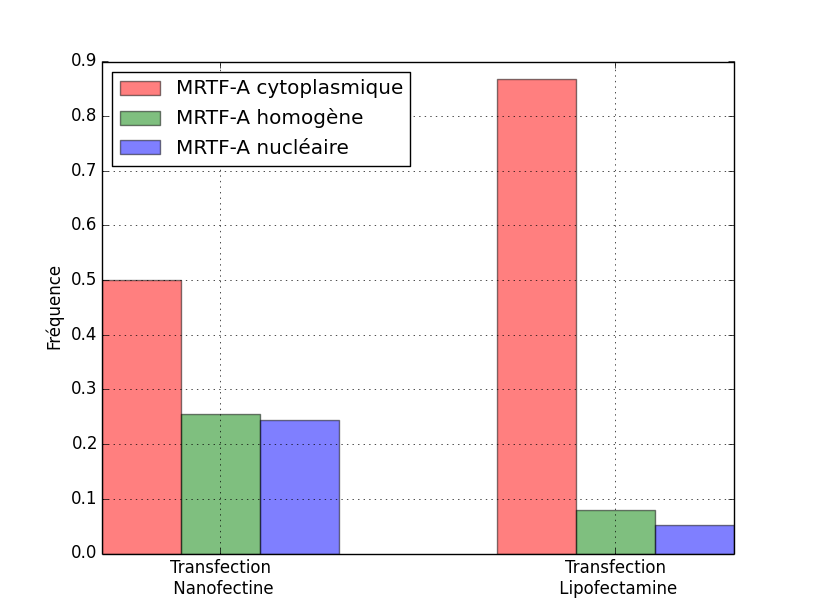
\includegraphics[scale=0.5]{Figures/Lipo_vs_Nano.png}
\caption{Comparaison de l'état après 20 minutes d'étirement (dont nous avons vu précédemment qu'il est proche de l'état initial) pour des C2C12 étirées à 10\% transfectées à la nanofectine (90 cellules en 5 expériences) ou à la lipofectamine (70 cellules en 4 expériences).  \label{LipoNano}}
\end{figure}

\begin{figure}[p]
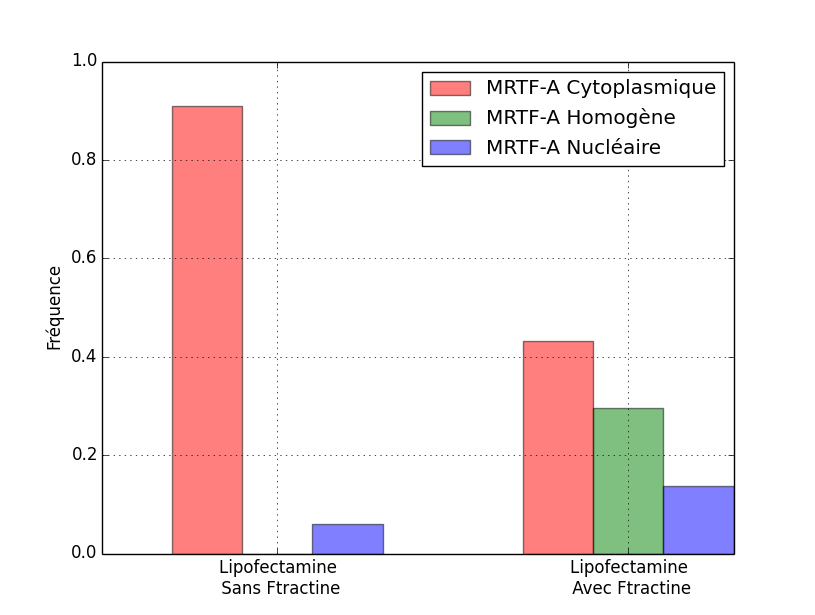
\includegraphics[scale=0.4]{Figures/Ftractine.png} 
\caption{Population initiale de cellules ayant MRTF-A cytoplasmique, homogène ou nucléaire, pour des C2C12 d'une même expérience, transfectées MRTF-A GFP et exprimant ou non la F-tractin RFP. \label{Ftractin}}
\end{figure}
\clearpage

\begin{figure}[p]
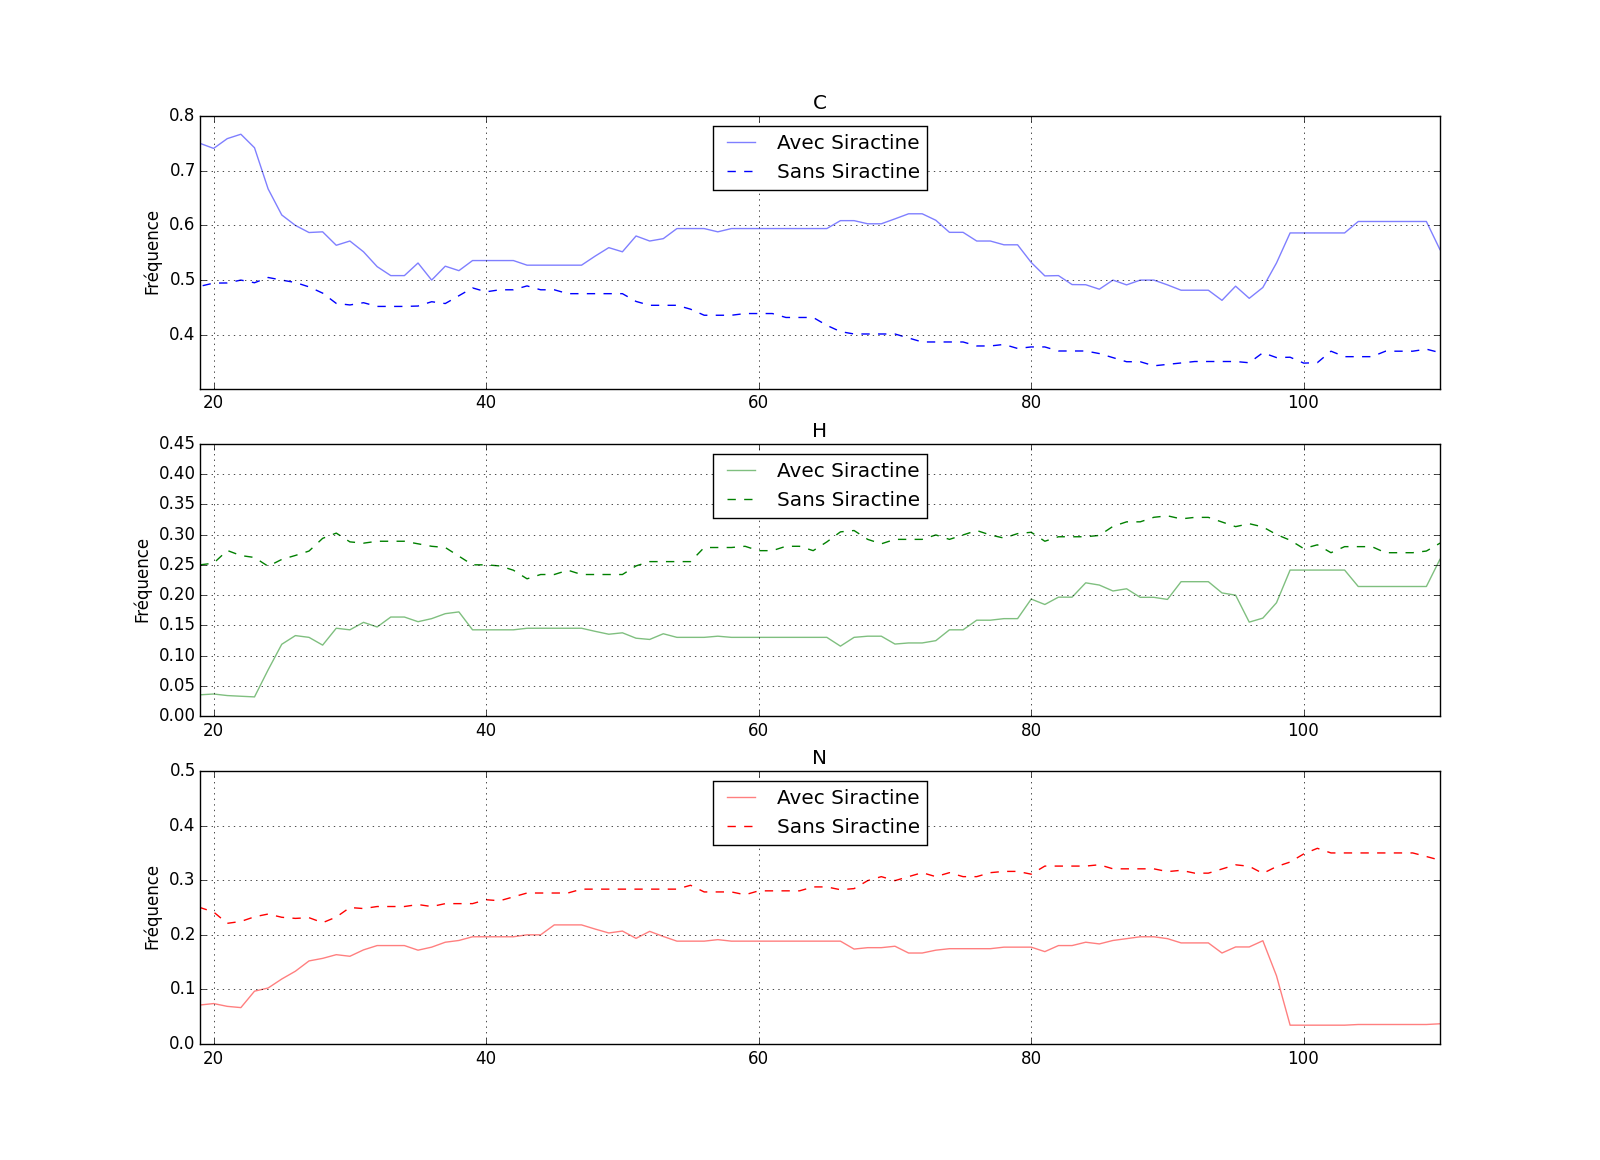
\includegraphics[scale=0.3]{Figures/Et10_Siractine_comparaison.png}
\caption{\'Evolution de la population de cellules ayant MRTF-A cytoplasmique, homogène ou nucléaire en fonction du temps écoulé depuis le début de l'étirement à 10\%, pour des C2C12 transfectées MRTF-A GFP avec de la nanofectine, et pour des C2C12 transfectées MRTF-A GFP avec de la lipofectamine et avec ajout de SiRactine pour visualiser les filaments d'actine. \label{CHN_SiR}}
\end{figure}

\begin{figure}[p]
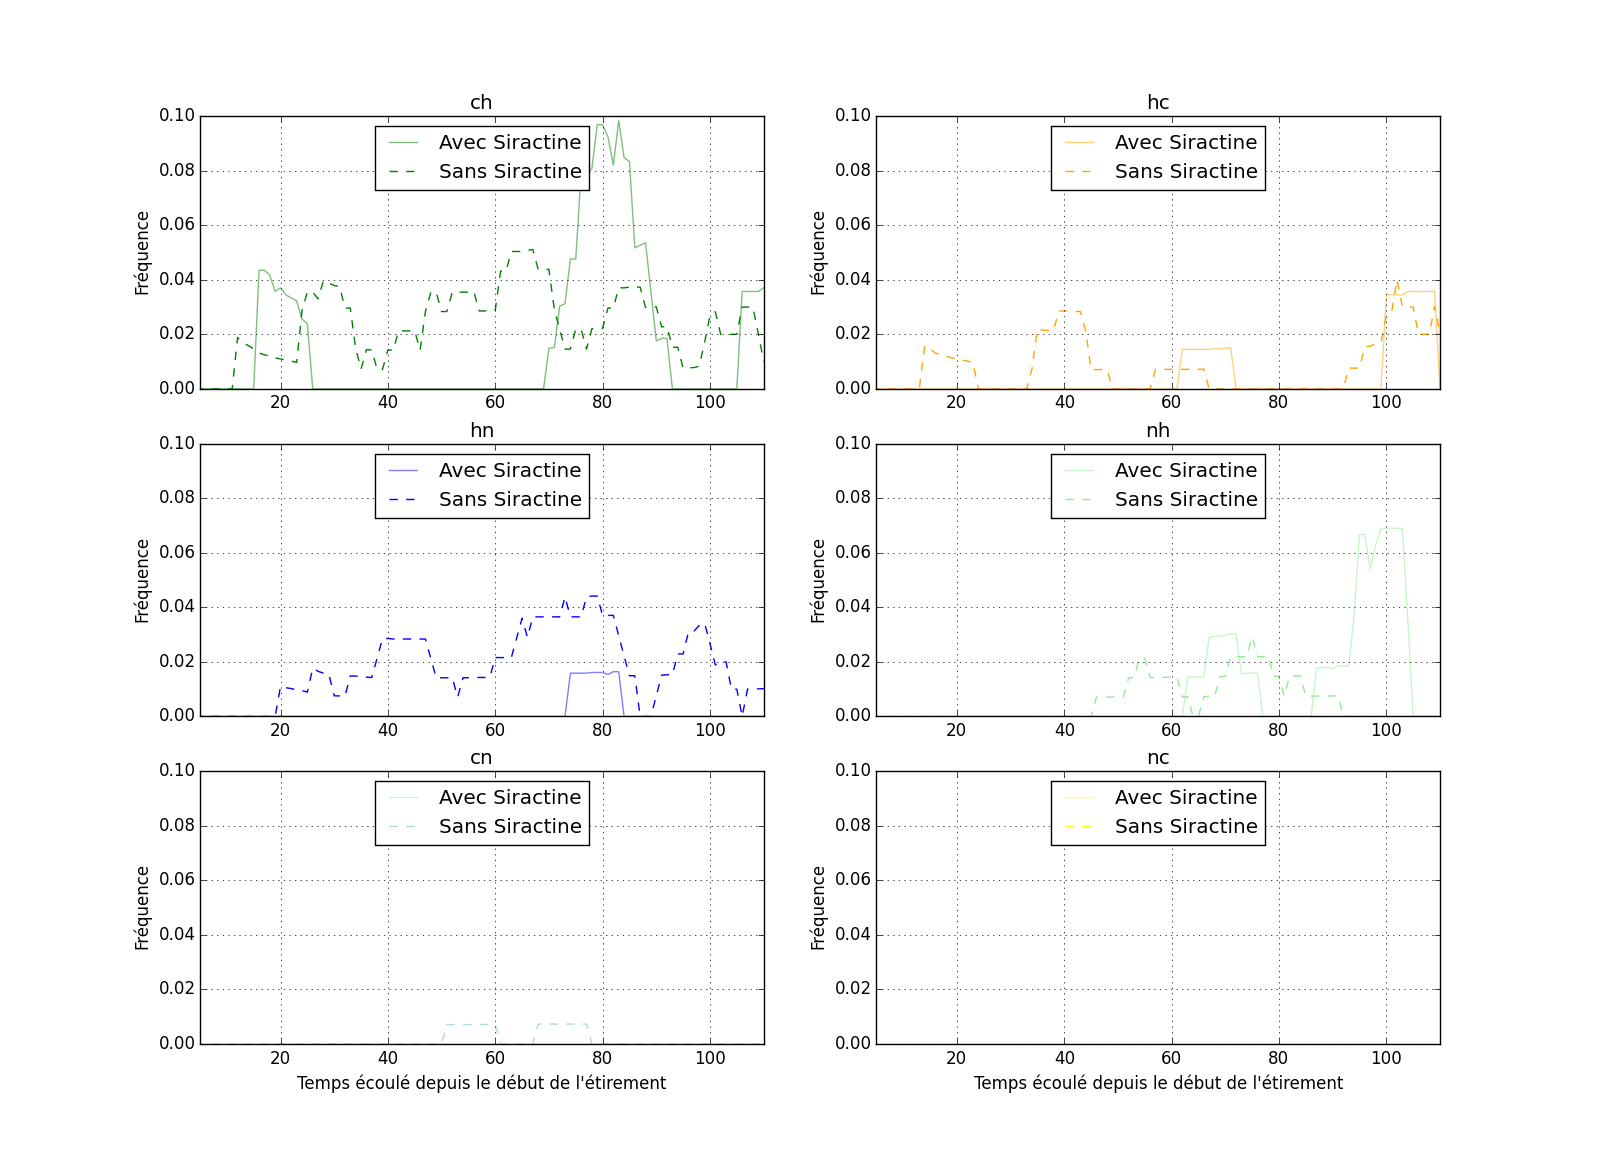
\includegraphics[scale=0.3]{Figures/Et10_transloc_Siractine.png} 
\caption{Nombre d'évènements ayant eu lieu pendant la fenêtre [t-5min,t+5min] pour chaque type de transition possible divisé par le nombre de cellules observées, pour des C2C12 transfectées MRTF-A GFP à la nanofectine et pour des C2C12 transfectées MRTF-A GFP à la lipofectamine et avec ajout de SiRactine, toutes étirées à 10\%. \label{transloc_Sir}}
\end{figure}

\begin{figure}[p]
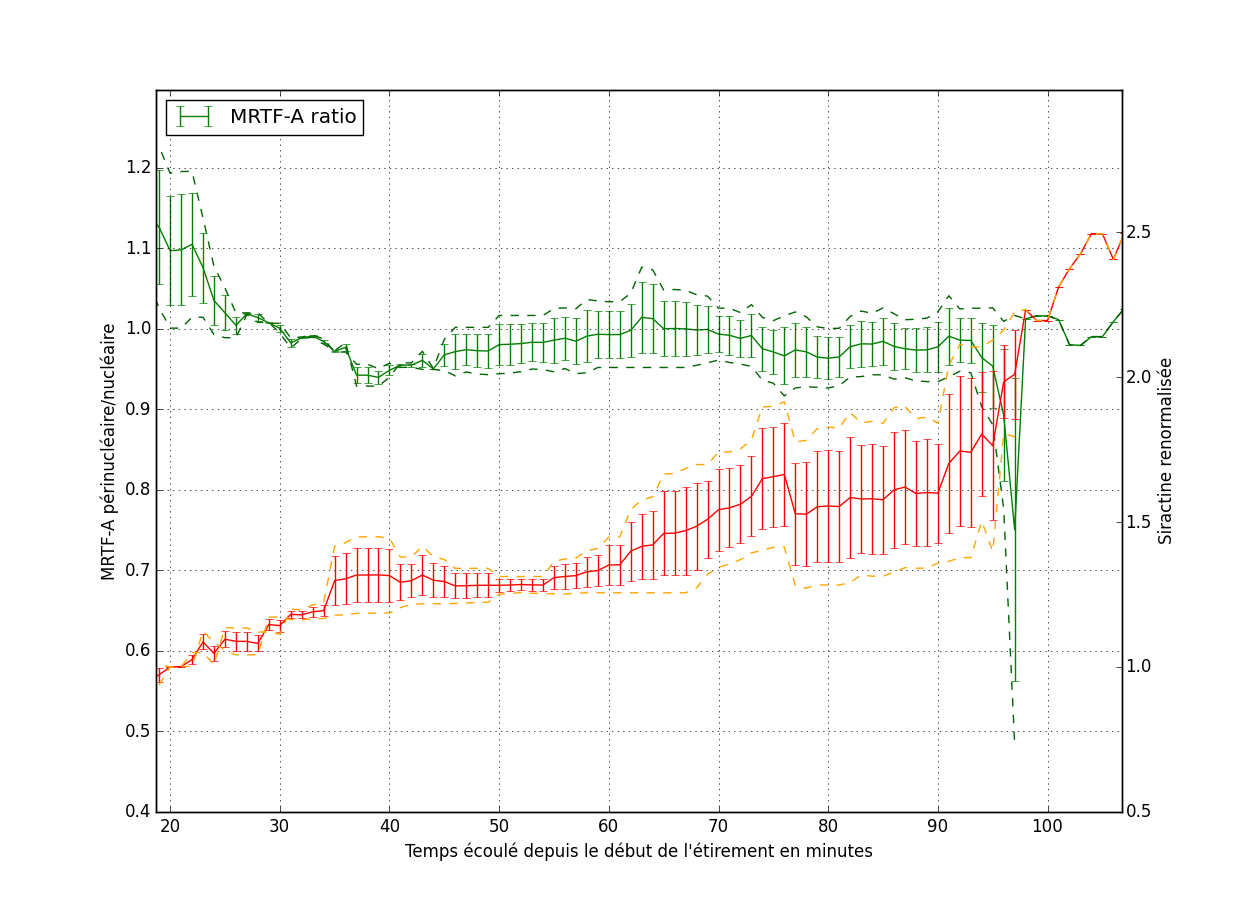
\includegraphics[scale=0.4]{Figures/C2C12.png} 
\caption{Ratio des intensités médianes de MRTF-A GFP péri-nucléaire/nucléaire (en vert) et Intensité médiane de SiRactine renormalisée par l'intensité médiane à 20 minutes (en rouge)  en fonction du temps écoulé depuis le début de l'étirement 10 \% (2 expériences, 68 cellules, les tracés en poitillés représentent chacune des deux expériences).\label{Siractine_quantif}}
\end{figure}

\begin{figure}[p]
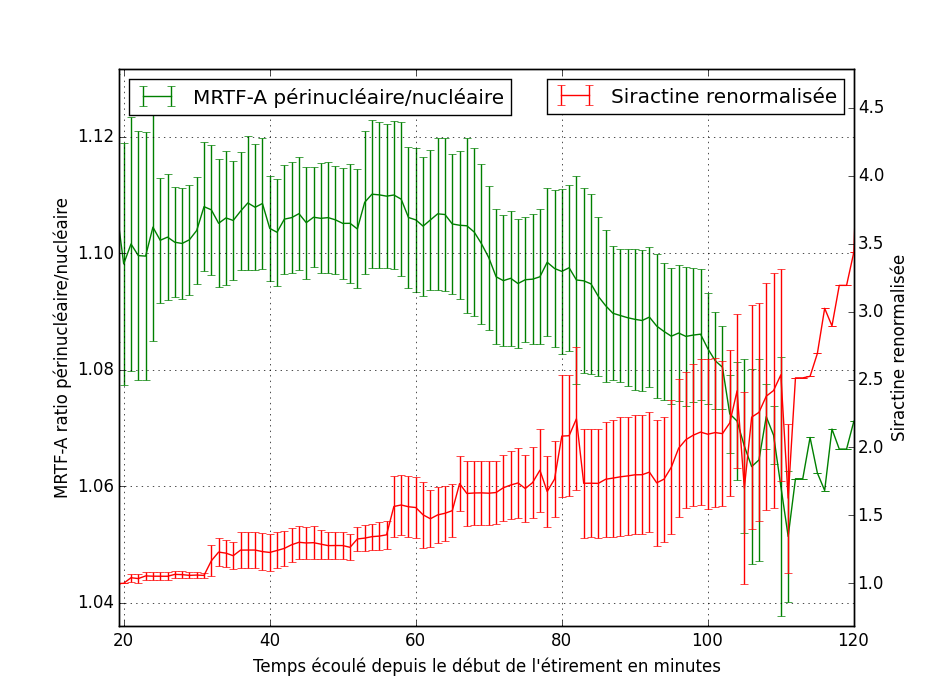
\includegraphics[scale=0.4]{Figures/Siractine_MRTFA_vs_temps.png} 
\caption{Rapport des intensités médianes en MRTF-A GFP  péri-nucléaire/nucléaire et Intensité en Siractine normalisée en fonction du temps écoulé depuis le début de l'étirement pour des myoblastes primaires soumis à 10\% d'étirement (5 expériences, 159 cellules). \label{myoblastes_Sir}}
\end{figure}

\begin{figure}[p]
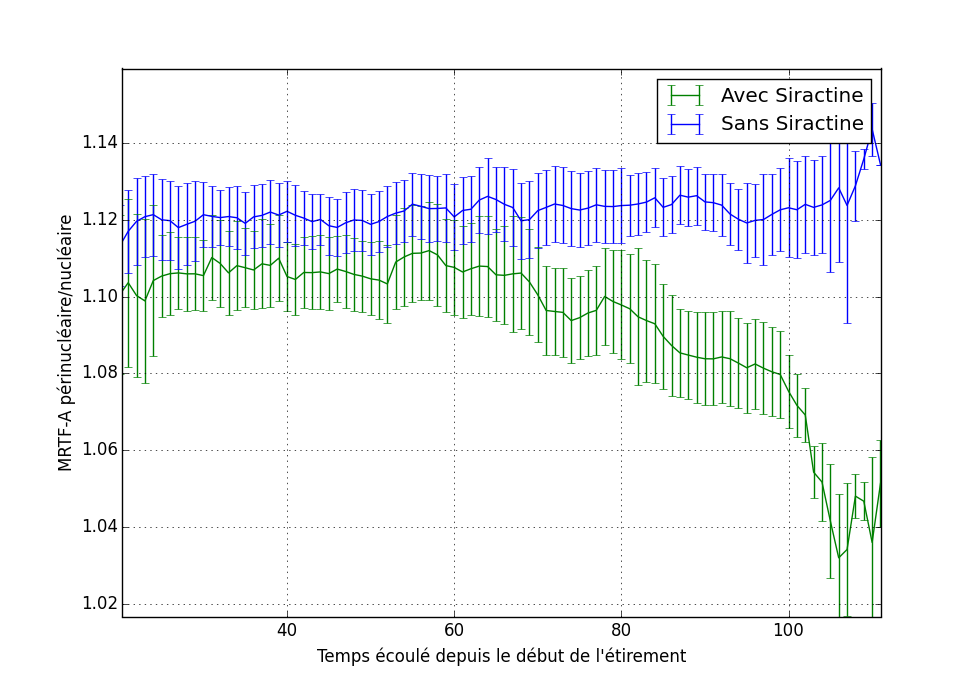
\includegraphics[scale=0.4]{Figures/Avec_Sans_Siractine.png} 
\caption{Rapport des intensités médianes en MRTF-A GFP  péri-nucléaire/nucléaire en fonction du temps écoulé depuis le début de l'étirement pour des myoblastes primaires soumis à 10\% d'étirement avec et sans ajout de SiRactine (Avec SiRactine : 5 expériences, 159 cellules, Sans SiRactine : 5 expériences, 239 cellules)}
\end{figure}

\begin{figure}[p]
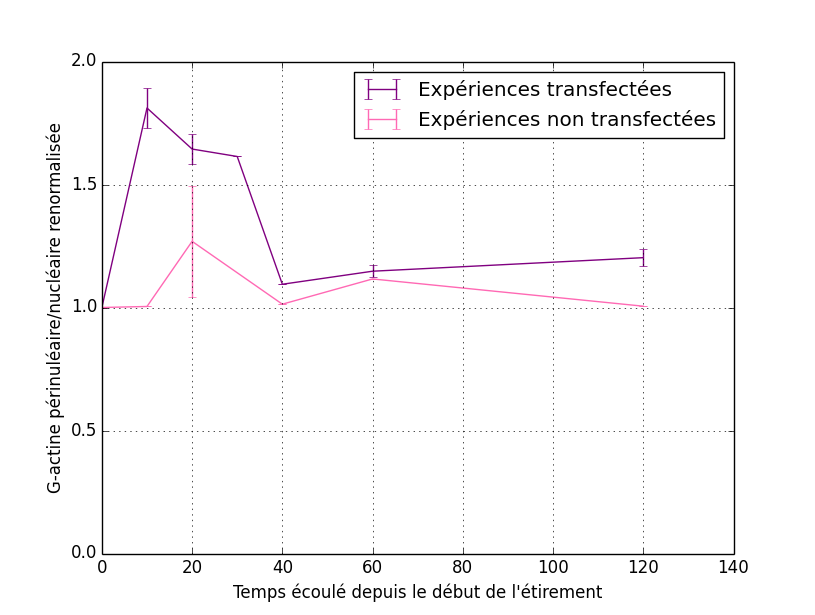
\includegraphics[scale=0.5]{Figures/Et10_G_ratio.png} 
\caption{\label{Et10_G} Intensité médiane du signal en DNase I (G-actine) dans la zone périnucléaire par rapport à la zone nucléaire, pour deux expériences sur des cellules MRTF-A GFP et deux expériences sur des cellules MRTF-A endogène, étirées à 10\%. Les données sont normalisées par la valeur au temps t=0, pour enlever les variations dues à la qualité du marquage d'une expérience à l'autre.}
\end{figure}

\begin{figure}[p]
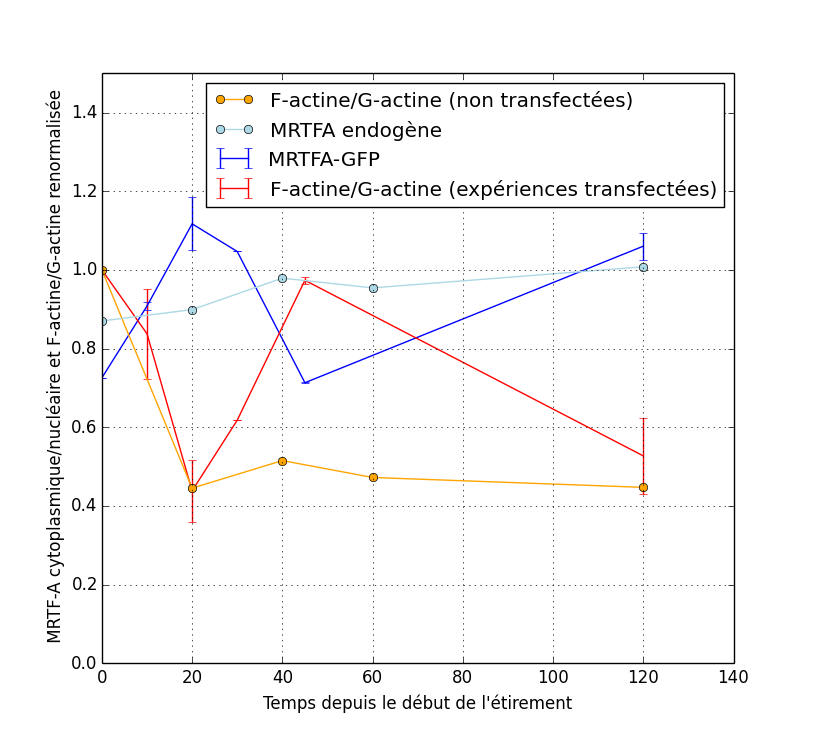
\includegraphics[scale=0.5]{Figures/Et30_MRTFA_FG.png} 
\caption{\label{Et30_MRTFA_FG} Intensité médiane de MRTFA-GFP ou de MRTF-A endogène dans la zone péri-nucléaire par rapport à la zone nucléaire (en bleu) et intensité médiane de la phalloïdine (F-actine) par rapport à la DNaseI (G-actine) (en rouge et orange)  au cours du temps, pour trois expériences transfectées et une non tranfectée, étirées à 30\%.  }
\end{figure}

\begin{figure}[p]
\includegraphics[scale=0.5]{Figures/Et30_Aires.png} 
\caption{\label{Et30_Aires} Aire moyenne des cellules au cours du temps pendant l'étirement 30\%. }
\end{figure}




\end{document}
